%!TEX root = ../my_thesis.tex
\chapter{Architecture matérielle de correction des erreurs résiduelles}

Dans le chapitre précédent, un algorithme permettant la correction des erreurs résiduelles a été présenté. Le quatrième 
chapitre
étudie l'implémentation matérielle de cet algorithme. Puisque ce dernier doit être interfacé avec un
turbo décodeur, il est nécessaire dans un premier temps d'étudier les architectures matérielles des turbo décodeurs
existantes dans la littérature. 

Suite à cela, dans un but d'adéquation entre l'algorithme et l'architecture, l'influence des différents paramètres 
de l'algorithme FNC sur les performances de décodage sera étudiée. Ceci afin d'identifier le meilleur compromis entre la
complexité calculatoire et le gain en correction d'erreurs résiduelles.

Enfin, un cas d'étude sera considéré afin de proposer une architecture matérielle de correction des erreurs résiduelles.
Des résultats d’implémentation sur cible FPGA illustreront la complexité matérielle de cette architecture.
Ce chapitre se terminera sur des propositions d'adaptations à réaliser pour
pouvoir adresser un très large spectre de turbo décodeurs.

\vspace*{\fill}
\minitocTITI
\vspace*{\fill}
\newpage

\section{Les architectures matérielles de turbo décodeurs}
Dans cette section, un état de l'art des architectures de turbo décodeurs est mené. Dans un premier temps, des détails 
sont donnés pour des architectures basées sur un processus itératif de turbo décodage séquentiel. Des architectures 
matérielles pouvant réaliser parallèlement plusieurs demi-itérations seront présentées dans un second temps.

\subsection{Traitement itératif séquentiel}
Le décodage des turbo codes est basé sur un échange d'informations extrinsèques entre différentes instances de décodage SISO. À partir 
des informations du canal et des informations \textit{a priori}, chaque instance de décodage SISO évalue les informations 
\textit{a posteriori}. De là, les informations extrinsèques sont déduites. Ces dernières sont alors utilisées en tant
qu'informations \textit{a priori} lors de la demi-itération suivante conjointement avec les informations de l'autre
domaine. La Figure \ref{fig:turbo_seq} présente la séquentialité de ces opérations lors du processus de décodage
itératif. Dans ce cas, un seul décodeur SISO effectue toutes les instances de décodage.
%Au cours des itérations, cet unique décodeur 

\begin{figure}[!h]
	\centering
	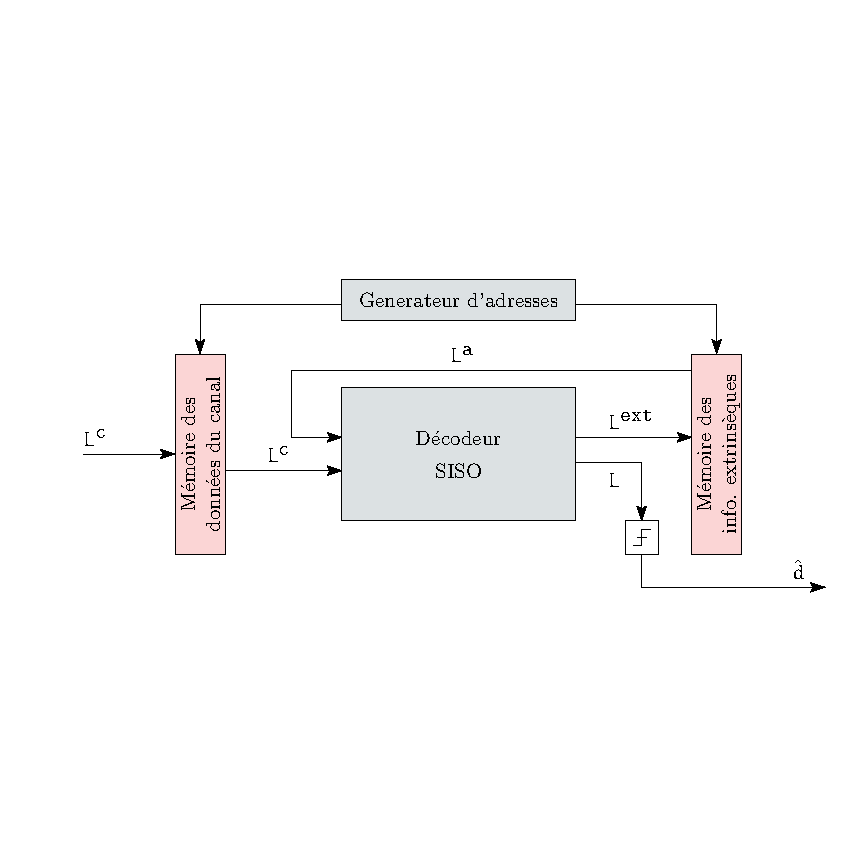
\includegraphics{main/ch4_fig/ipe/serial.pdf}
	\caption{Principe du turbo décodage séquentiel. \label{fig:turbo_seq}}
\end{figure} 

Dans les architectures matérielles de turbo décodeurs, l'algorithme de décodage SISO choisi pour l’obtention des informations \textit{a posteriori} est l'algorithme MAP, 
ou plutôt une des ses simplifications, à savoir l'algorithme EML-MAP. Cet algorithme repose sur trois calculs successifs et 
séquentiels. Suivant l'ordonnancement choisi et le degré de parallélisme retenu pour ces calculs, différentes valeurs 
au niveau des ressources calculatoires, de mémorisation et des temps d'exécutions sont obtenues. Une description
incrémentale des différentes approches de l'implémentation du décodeur SISO est maintenant menée, suivant la 
classification proposée dans \cite{Muller2010}.

\subsubsection{Traitement séquentiel de l'algorithme BCJR}
\paragraph*{BCJR aller-retour}
Les étapes de l'algorithme BCJR sont détaillées ci-après. Tout d'abord, le calcul des métriques de branches, notées 
$\gamma$, est effectué. Ceci permet d’initier le calcul récursif des métriques de nœuds aller, notées $\alpha$. Chaque 
métrique de nœud aller est calculée en combinant la transition courante du treillis avec les métriques $\alpha$ de la 
section de treillis précédente. Le calcul récursif des métriques de nœuds retour, notées $\beta$, est similaire mais
considère un parcours du treillis %du code 
dans l'autre sens, en partant de la fin du treillis. Finalement, les 
informations \textit{a posteriori} sont calculées en combinant les trois métriques $\alpha$, $\beta$ et $\gamma$. 

Comme dans le cas de l'algorithme de Viterbi, chaque calcul de métrique de nœud est réalisé par une opération ACS 
(Addition-Comparaison-Sélection). En allouant autant d'unités ACS qu'il existe de nœuds dans une section du treillis, 
il est possible de calculer parallèlement toutes les métriques de nœuds (aller ou retour) d'une même section. Ce
parallélisme ne nécessite que peu de surcoût matériel puisque seules les unités ACS sont dupliquées sans nécessiter
de mémoire additionnelle. En effet chaque opération ACS est exécutée sur le même ensemble de données. Ainsi, toutes les 
métriques de nœuds d'une section de treillis peuvent être calculées en un cycle d'exécution. Le calcul récursif des métriques de 
nœuds nécessite alors au total K cycles d'exécutions.

Dans ce contexte, un cycle d'exécution après le début du calcul des métriques de nœuds retour, il est possible d'effectuer le calcul de l'information 
\textit{a posteriori}. Cet ordonnancement des opérations correspond à celui originellement proposé par Bahl, Cocke, 
Jelinek et Raviv lors de la présentation de leur algorithme de décodage \cite{bcjr}. Dans le suite du manuscrit, cet
ordonnancement des opérations est nommé Forward-Backward (FB). Il est schématisé dans la Figure \ref{fig:siso_seq}.
Il apparaît que le temps requis pour exécuter une demi-itération du processus de décodage itératif équivaut à $2\times K$ cycles d'horloge. Dans le cadre du standard LTE, à cause des bits de terminaisons de treillis, cette durée est légèrement
plus importante en réalité. Cependant, afin d'exprimer plus simplement le nombre de cycles nécessaires, le temps de 
traitement des bits de terminaison n'est jamais pris en compte dans ce chapitre.
Pour pouvoir disposer des informations 
\textit{a posteriori}, la mémorisation des K métriques de nœuds aller est requise. 

\begin{figure}[!h]
	\centering
	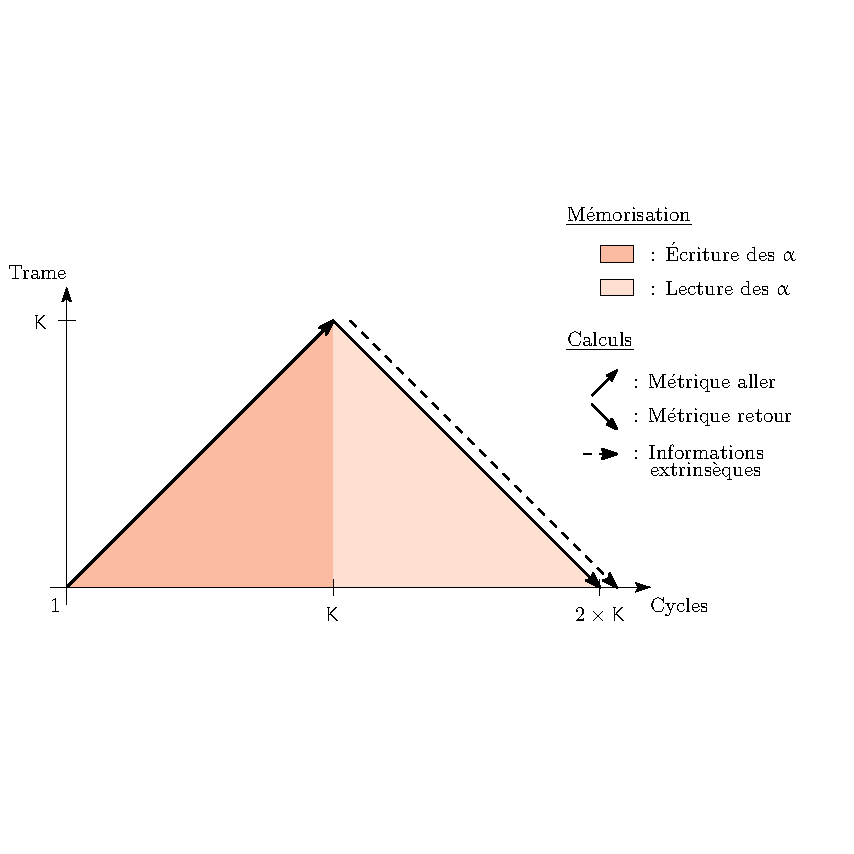
\includegraphics{main/ch4_fig/ipe/FB+LEG_2.pdf}
	\caption{Ordonnancement BCJR Aller-Retour (FB). \label{fig:siso_seq}}
\end{figure}

\paragraph*{BCJR aller-retour à l'aide d'une fenêtre glissante}
La technique de fenêtre glissante (sliding-window) a été proposée pour faciliter le traitement associé à un ordonnancement
FB. L'objectif réside en
la réduction de la quantité de données à mémoriser. Son principe est le suivant. La trame à décoder est découpée en W fenêtres 
de tailles $\frac{K}{W}$. Après avoir calculé K/W métriques de nœuds aller, le calcul des métriques de nœuds retour débute à l'index K/W. 
Lors du cycle d'exécution suivant, le calcul des informations \textit{a posteriori} est initié. À la fin de la 
récursion retour, le traitement est appliqué à une autre fenêtre de la trame. Ce procédé est répété W fois, jusqu'à ce que l'ensemble de la trame
soit traitée. Les besoins de mémorisation se limitent alors à K/W métriques de nœuds aller.
Cependant, la suppression de la 
récursion aux limites des fenêtres introduit une dégradation au niveau des performances de décodage. Pour palier ce problème, deux 
techniques ont été proposées. Il s'agit de l'utilisation : 
\begin{itemize}
	\item d'une fenêtre d'acquisition. Dans ce cas, le calcul des métriques de nœuds retour est appliqué sur 
	quelques sections de treillis autour de la fenêtre. Une étude empirique a montré que la 
	taille de prologue ayant le meilleur compromis entre calculs supplémentaires et gain de 
	décodage se situe entre 3 et 5 fois la longueur de contrainte du code constituant \cite{sw_init}.
	\item du passage de messages. Son principe consiste à utiliser les métriques de nœuds calculées lors de l'itération 
	précédente comme valeurs initiales pour les limites de la fenêtre. Cette technique propose de meilleurs 
	performances de décodage que la technique de la fenêtre d'acquisition pour un surcoût de mémorisation limité \cite{muller2006}.\vspace*{1ex}
\end{itemize}

Si l'ordre des calculs est inversé, c'est-à-dire si en premier lieu le calcul des métriques de nœud retour est 
effectué, il est possible de produire les informations extrinsèques dans l'ordre croissant en n'utilisant que $K/W + K$
cycles. Dans ce cas, les unités de calcul de nœuds aller et retour doivent fonctionner en même temps. Ceci ne 
nécessite pas de ressources matérielles supplémentaires puisqu'elles sont déjà présentes dans le cas de l'ordonnancement 
FB. Les besoins en mémorisation sont en revanche réduits à $K/W$ données. Cet ordonnancement est nommé dans la suite 
Backward-Forward-Sliding-Window (BF-SW). La Figure \ref{fig:siso_sw} schématise un tel ordonnancement pour $W=2$.

\begin{figure}[!hb]
	\centering
	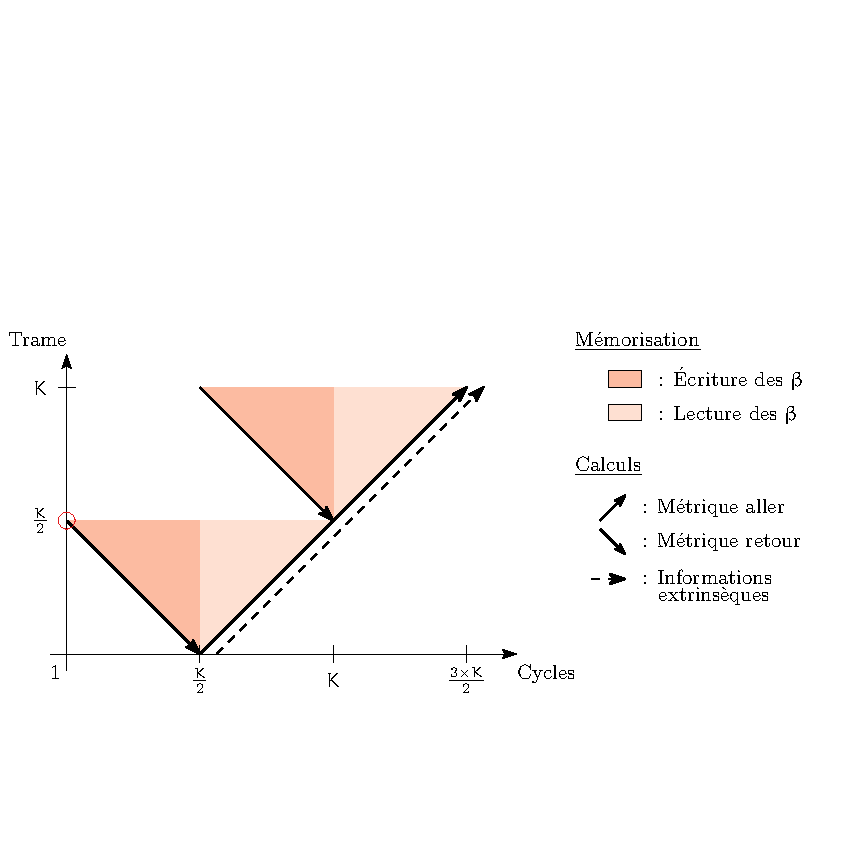
\includegraphics{main/ch4_fig/ipe/BF_SW+LEG.pdf}
	\caption{Ordonnancement BCJR Retour-Aller avec fenêtre glissante, W=2 (BF-SW). \label{fig:siso_sw}}
\end{figure}

\subsubsection{Traitement parallèle de l'algorithme BCJR}
\paragraph*{BCJR en ailes de papillon}
À partir de l'ordonnancement BF-SW, en ne considérant qu'une seule fenêtre mais en doublant le nombre d'unités de 
calcul d'information \textit{a posteriori}, il est possible de débuter les calculs récursifs des métriques de nœuds 
aller et des métriques de nœuds retour au même cycle. Dans ce cas, à partir de la moitié du parcours du treillis, deux 
informations extrinsèques sont produites durant chaque cycle d'exécution. Cet ordonnancement est nommé BCJR en ailes de papillon (butterfly, 
abrégé en BFLY dans la suite) \cite{butterfly}. Il est illustré par la Figure \ref{fig:siso_but}. De la sorte, seuls 
$K$ cycles d'exécution sont nécessaires pour effectuer une demi-itération de turbo décodage. Le nombre de données à mémoriser
est similaire à celui de l'ordonnancement BCJR aller-retour. En revanche, les informations extrinsèques sont produites par paires à 
partir du $K/2^{\text{ième}}$ cycle d’exécution. Cet ordonnancement permet donc de réduire le temps de traitement du turbo décodage d'un 
facteur deux par rapport à l'ordonnancement FB.

\begin{figure}[h]
	\centering
	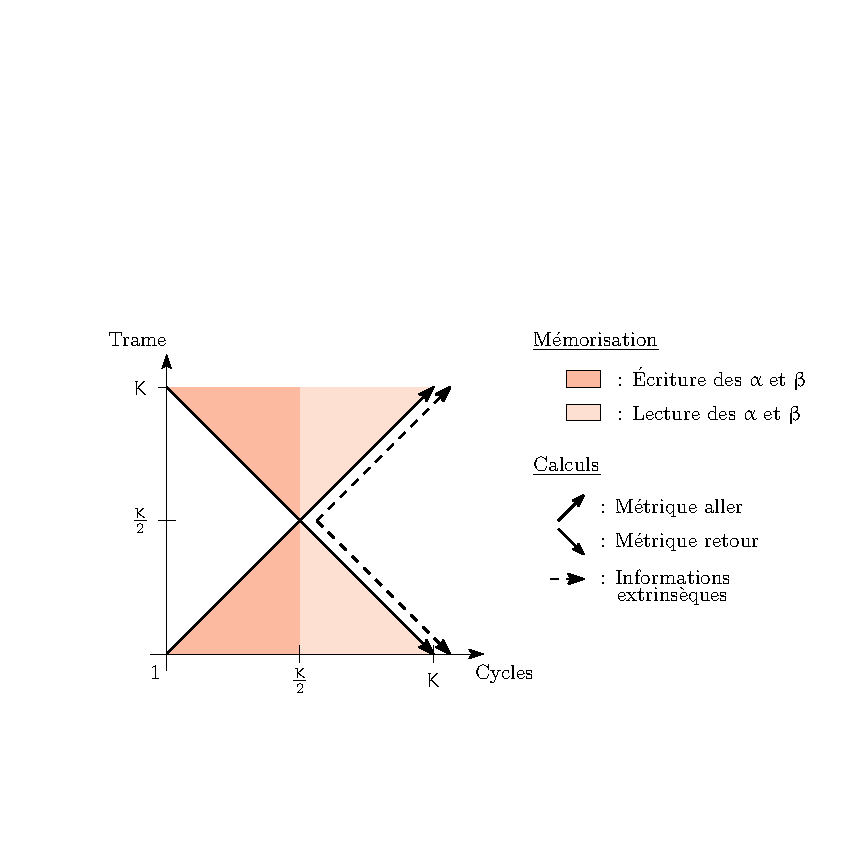
\includegraphics{main/ch4_fig/ipe/BFLY+LEG.pdf}
	\caption{Ordonnancement BCJR Butterfly (BFLY). \label{fig:siso_but}}
\end{figure}

\paragraph*{BCJR en ailes de papillon à l'aide d'une fenêtre glissante}
Toujours dans un but de réduire le nombre de données à mémoriser, il est possible d'utiliser le concept de fenêtre 
glissante conjointement à l'ordonnancement BFLY. Comme pour l'ordonnancement FB, le découpage de la trame en W fenêtres 
permet de réduire les ressources de mémorisation d'un facteur W. Cependant, dans ce cas, aucun gain en latence n'est obtenu. La Figure \ref{fig:siso_bf_sw} détaille cet ordonnancement (abrégé en BFLY-SW) pour $W = 2$. Dans ce cas, 
les informations extrinsèques sont produites par paires durant deux intervalles de temps ayant pour durée K/4 cycles 
d'exécution.


\begin{figure}[!h]
	\centering
	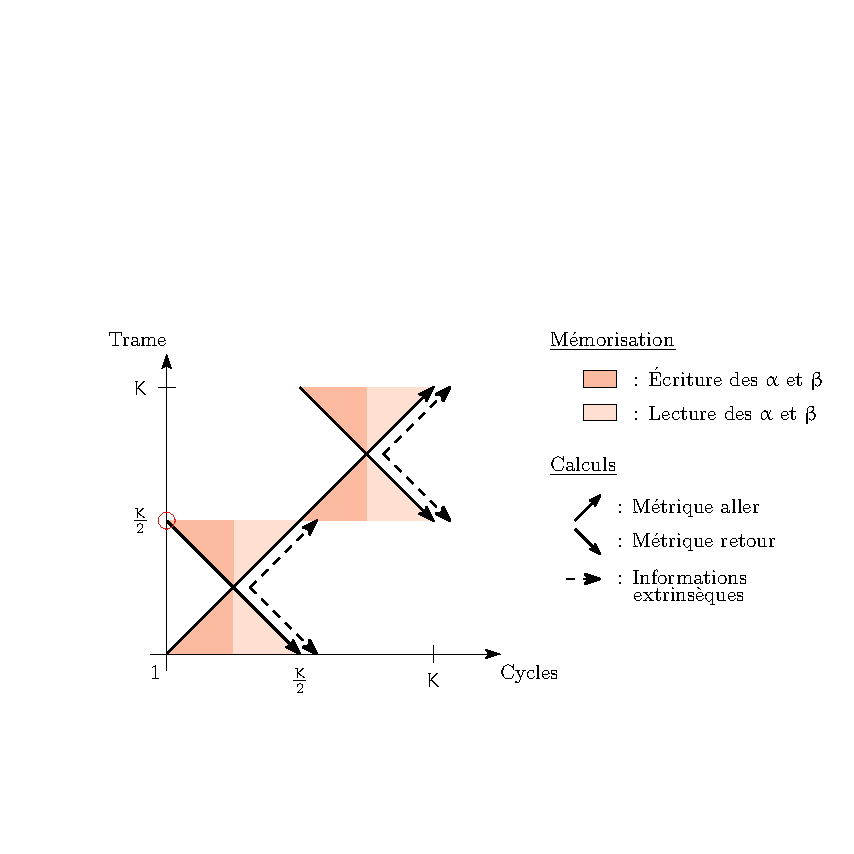
\includegraphics{main/ch4_fig/ipe/BFLY_SW+LEG.pdf}
	\caption{Ordonnancement BCJR Butterfly avec fenêtre glissante (BFLY-SW). \label{fig:siso_bf_sw}}
	\vspace*{-1ex}
\end{figure}

% \begin{figure}[!h]
%     \centering
%     \begin{minipage}[t]{.49\textwidth}
% 	\centering
% 	\includegraphics{main/ch4_fig/ipe/BFLY.pdf}
% 	\caption{Ordonnancement BCJR Butterfly (BFLY). \label{fig:siso_but}}
%     \end{minipage}~~~~~~%
%     \begin{minipage}[t]{0.49\textwidth}
% 	\centering
% 	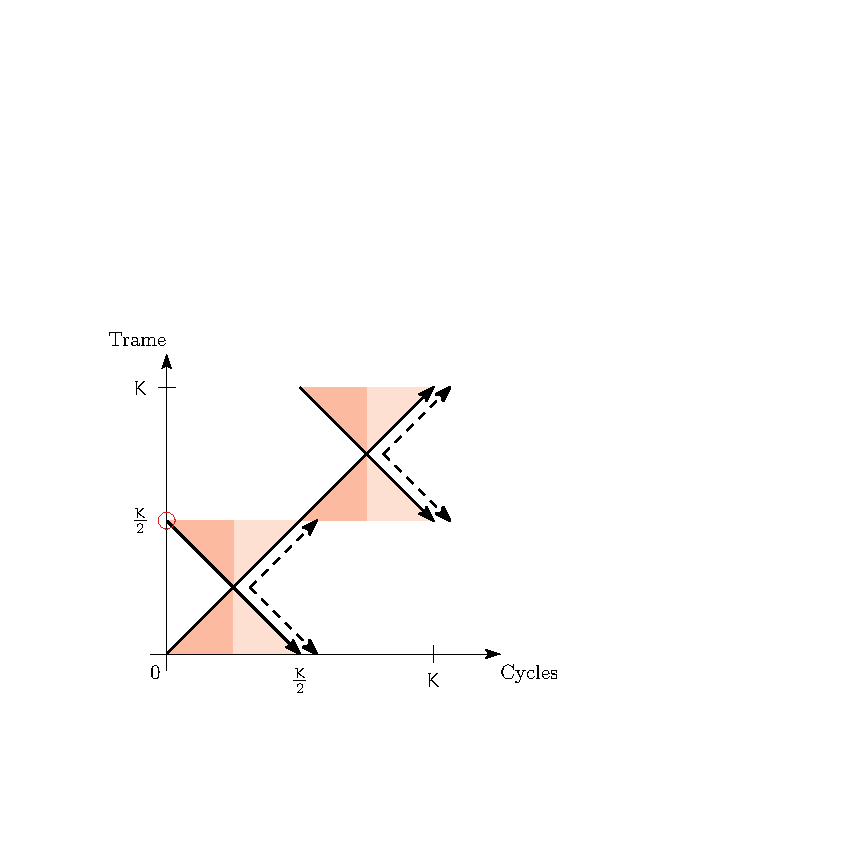
\includegraphics{main/ch4_fig/ipe/BFLY_SW.pdf}
% 	\caption{Ordonnancement BCJR Butterfly avec fenêtre glissante (BFLY-SW). \label{fig:siso_bf_sw}}
%     \end{minipage}
% \end{figure}

\subsection{Parallélisme au sein du processus itératif}
Il est aussi possible d'agir sur d'autres niveaux de parallélisme en plus de celui concernant l'ordonnancement des traitements
de l'algorithme BCJR. Tout d'abord un 
parallélisme opérant au niveau du calcul d'une demi-itération est présenté.
\subsubsection{Parallélisme au sein d'une demi-itération}
À partir de l'algorithme basé sur une fenêtre glissante, afin de gagner un niveau de parallélisme supplémentaire, il est possible 
d'augmenter le nombre de décodeurs SISO. Chaque décodeur opère alors sur une fenêtre différente de la 
trame. La Figure \ref{fig:turbo_par} illustre un tel degré de parallélisme pour un nombre de sous blocs de deux ($B=2$).
Dans ce cas, deux décodeurs SISO se répartissent le traitement de la trame. Un décodeur SISO s'occupe des informations allant de l'index
1 à K/2 et le second de l'index K/2+1 à K. Là encore, une initialisation aux limites des sous-trames s'avère nécessaire. Les mêmes 
techniques que présentées précédemment peuvent être envisagées. Cependant, cette fois, en plus des métriques de nœuds
retour, les métriques de nœuds aller doivent aussi être considérées. Aussi ce degré de parallélisme implique que 
l'entrelaceur puisse lui aussi être parallélisé afin qu’aucun conflit d'accès ne puisse apparaître 
\cite{interleaver_conflict}. 
La temps nécessaire pour effectuer une demi-itération est alors réduit d'un facteur $B$. Cependant, les ressources 
calculatoires associées aux décodeurs SISO sont multipliées par ce même facteur.

\begin{figure}[!h]
	\centering
	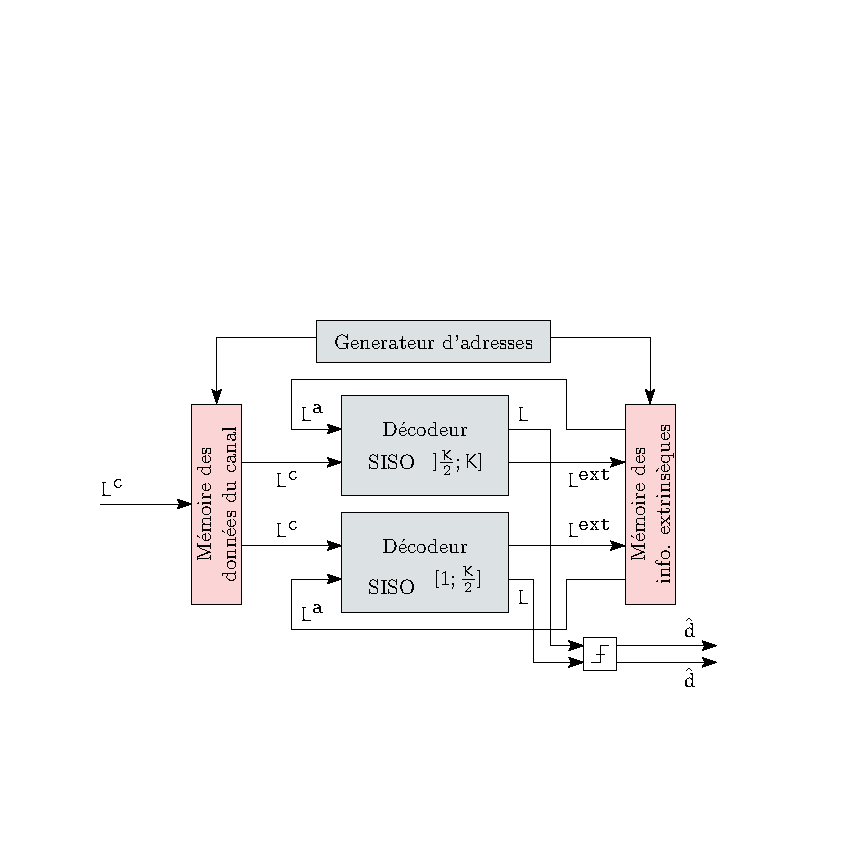
\includegraphics{main/ch4_fig/ipe/parallel_2.pdf}
	\caption{Principe de turbo décodage basé  sur plusieurs décodeurs SISO. \label{fig:turbo_par}}
\end{figure} 

Le choix de l'ordonnancement au sein de chaque décodeur SISO n'est pas contraint. La Figure \ref{fig:sisos_par} présente un niveau de 
parallélisme de 2 associé à l'ordonnancement BFLY pour un nombre de sous-blocs valant 2. Cet ordonnancement est nommé 
BFLY-SB dans la suite. Il apparaît que dans ce cas, K/2 cycles d'exécution sont nécessaires pour effectuer une demi-itération. 
Durant les K/4 derniers cycles d'exécution, 4 informations extrinsèques sont produites en parallèle. Finalement, le nombre de
données à mémoriser est équivalent à celui d'un ordonnancement BFLY.

Afin de réduire les besoins en terme de mémorisation, il est possible de combiner le parallélisme de sous-blocs avec le principe 
de fenêtre glissante. De la sorte, en considérant W fenêtres différentes, la taille de la mémoire est réduite d'un 
facteur W au niveau des métriques de nœuds. La Figure \ref{fig:sisos_par_sb} présente un ordonnancement Butterfly avec 
2 fenêtres glissantes et un parallélisme de décodeurs SISO de 2. Cet ordonnancement est nommé BFLY-SB-SW dans la suite
du manuscrit.

% \begin{figure}[!h]
%     \centering
%     \begin{minipage}[t]{.49\textwidth}
%         \centering
%         \includegraphics{main/ch4_fig/ipe/BFLY_SB.pdf}
% 		\caption{Ordonnancement BCJR Butterfly en parallèle (BFLY-SB). \label{fig:sisos_par}}
%     \end{minipage}~~~~~~%
%     \begin{minipage}[t]{0.49\textwidth}
%         \centering
%         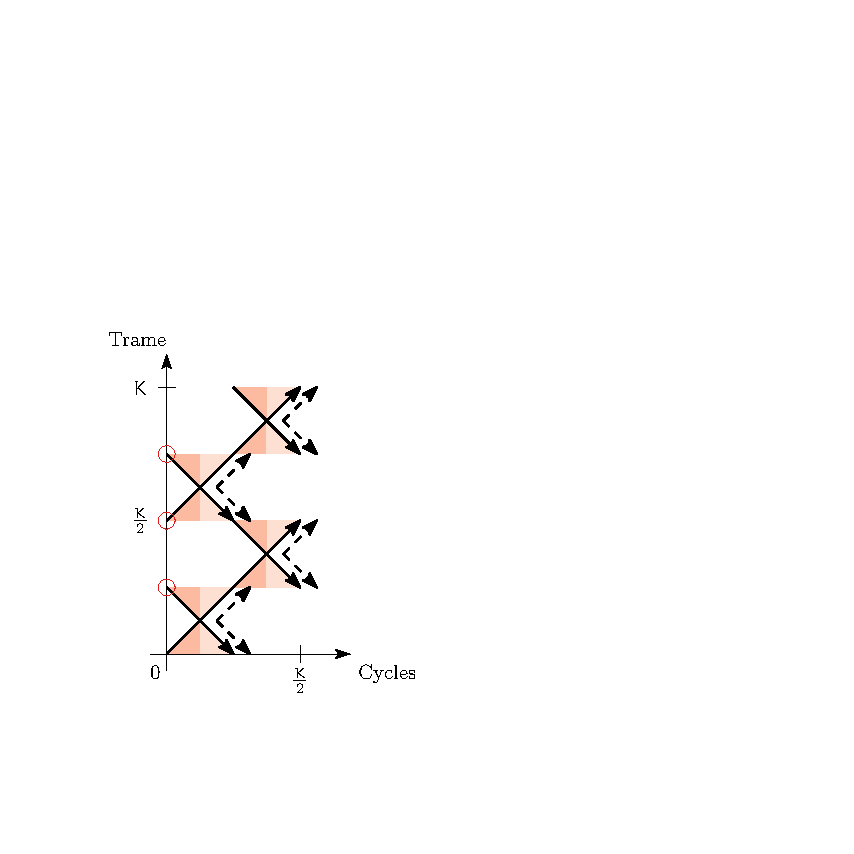
\includegraphics{main/ch4_fig/ipe/BFLY_SB_SW.pdf}
% 		\caption{Ordonnancement BCJR Butterfly avec fenêtre glissante en parallèle (BFLY-SW-SB). \label{fig:sisos_par_sb}}
%     \end{minipage}
% \end{figure}

\begin{figure}[!h]
    \centering
    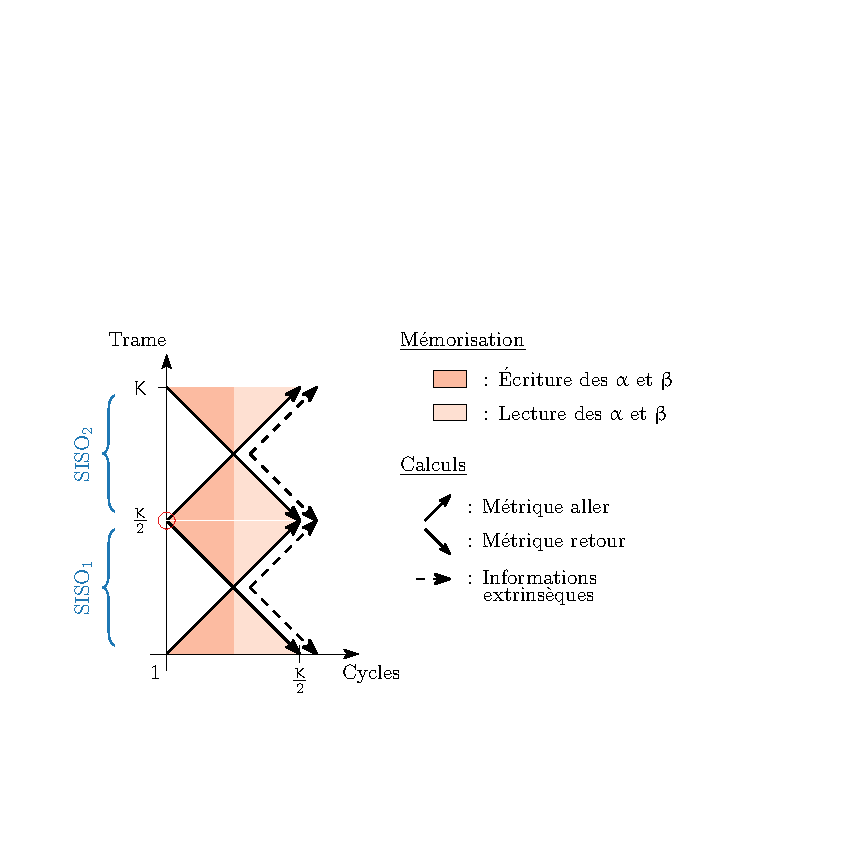
\includegraphics{main/ch4_fig/ipe/BFLY_SB+LEG.pdf}
	\caption{Ordonnancement BCJR Butterfly en parallèle (BFLY-SB). \label{fig:sisos_par}}
\end{figure}    
\begin{figure}[!h]
    \centering
    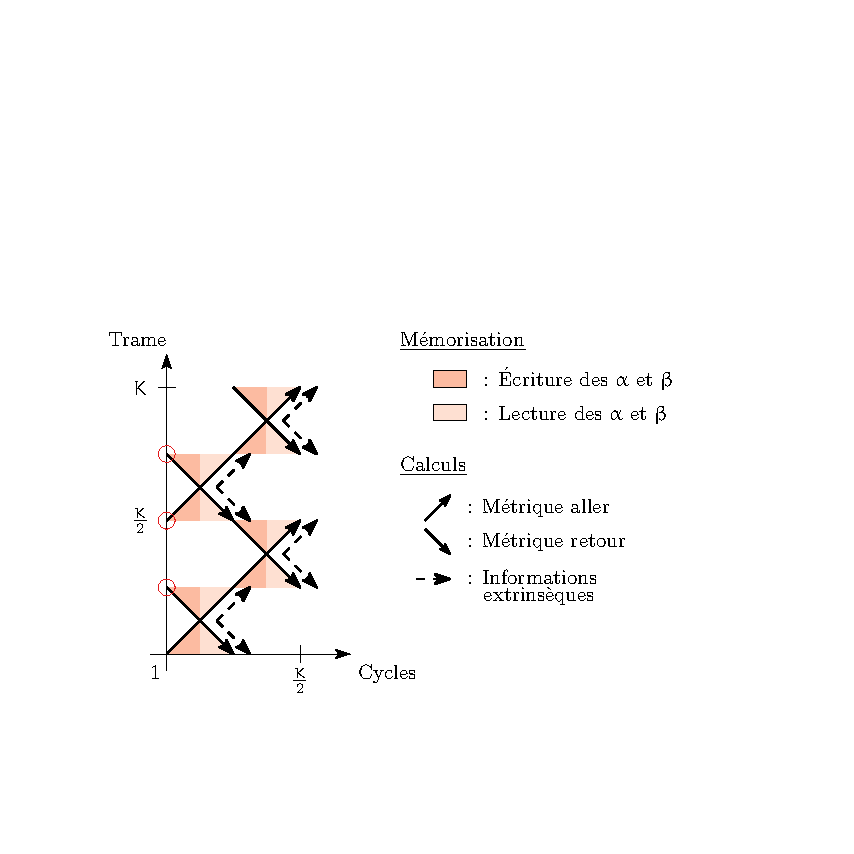
\includegraphics{main/ch4_fig/ipe/BFLY_SB_SW+LEG.pdf}
	\caption{Ordonnancement BCJR Butterfly avec fenêtre glissante en parallèle (BFLY-SW-SB). \label{fig:sisos_par_sb}}
\end{figure}

\subsubsection{Parallélisme de demi-itérations}
Plus encore, il est possible de considérer un autre niveau de parallélisme. Il est en effet possible de faire opérer le 
décodage des deux codes convolutifs élémentaires en même temps \cite{turbo_par}. Dans ce cas, après chaque itération, 
chaque décodeur élémentaire travaillant dans un certain domaine fourni ses informations extrinsèques au décodeur 
élémentaire utilisant les données du canal de l'autre dimension. Cependant, cette technique nécessite à performances de 
décodage égales deux fois plus d'itérations que le turbo décodage conventionnel. Ceci vient du fait que le principe 
itératif du turbo décodage conventionnel n'est plus respectée dans cette organisation.

Pour palier cela, en 2005, le décodage dit shuffled a été proposé \cite{turbo_shuff}. Dans ce cas,  les informations extrinsèques sont échangées entre les deux domaines dès qu'elles ont 
été calculées. Chaque décodeur composant dispose donc plus vite des information \textit{a priori} mises à jour avant la 
fin des traitements associés à la demi-itération courante. Ceci a 
alors pour effet d'augmenter la vitesse de convergence du turbo décodeur. 
%Dans ce cas, 
%et permet donc d'approcher les mêmes besoin en itération qu'avec
%un turbe décodage conventionnel pour des performances de décodage équivalentes. 
Il est cependant à noter que ceci est 
vrai avec un ordonnancement Butterfly-Replica \cite{butt_replica}. Ce dernier permet, au prix d'un doublement de 
la mémoire associée aux métriques de nœuds, de produire des informations extrinsèques durant toute la durée de la demi-itération. 
Cela participe à l'augmentation de la vitesse de convergence.
La Figure \ref{fig:turbo_shuff} présente un échange d'informations extrinsèques au cours du processus de décodage 
shuffled pour deux décodeurs composants travaillant en simultané.

Pour de telles implémentations de turbo décodeurs, une approche utilisant de multiples processeurs à jeu d’instructions 
spécifiques (ASIP) est à privilégier \cite{asip}.

\begin{figure}[!h]
	\centering
	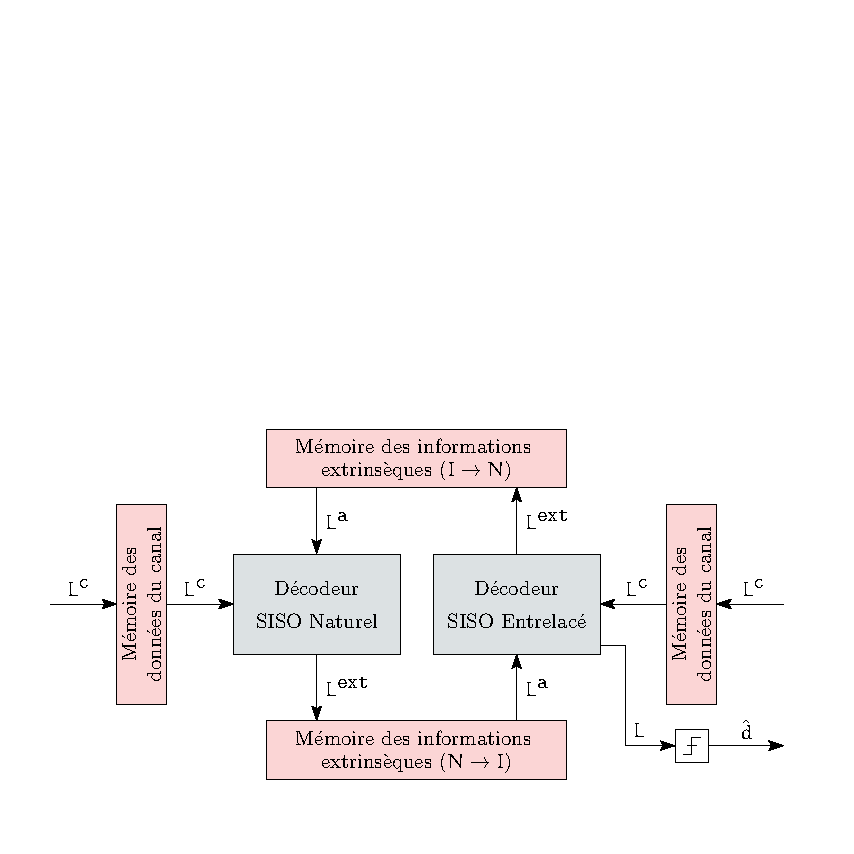
\includegraphics{main/ch4_fig/ipe/shuffled_2.pdf}
	\caption{Principe de turbo décodage Shuffled. \label{fig:turbo_shuff}}
\end{figure}

\subsubsection{Parallélisme de décodage entre différentes trames}
La dernière technique permettant d'augmenter l'efficacité du processus de décodage revient à dupliquer les décodeurs 
SISO au cours du traitement itératif. Ceci permet alors de décoder simultanément plusieurs trames. Cette méthode revient 
à utiliser une architecture pipeline pour le turbo décodeur. Ainsi des décodeurs SISO sont assignées à une ou plusieurs 
itérations. Cela implique une organisation pipeline pour mémoriser les trames entre les décodeurs SISO. Dans ce cas, la 
profondeur maximale du pipeline équivaut à deux fois le nombre maximal d'itérations. Bien que permettant une augmentation 
conséquente du débit, cette approche ne réduit pas la latence du processus de décodage. En revanche, elle s'avère 
coûteuse sur le plan matériel puisque toutes les ressources calculatoires et de mémorisation sont dupliquées P fois, 
avec P la profondeur du pipeline.

\subsection{Conclusion}
Dans cette première section, différentes organisations d'architectures matérielles dédiées au turbo décodage ont été présentées.
Différentes techniques visant à augmenter le parallélisme de calcul dans le processus de décodage ont été décrites. 
Elles favorisent une diminution de la 
latence globale du décodeur et/ou une réduction de la quantité de données à mémoriser. Néanmoins les gains s’obtiennent
aux dépens de la complexité calculatoire. De plus, elles impactent l'ordonnancement de la génération des informations 
\textit{a posteriori}. Une synthèse de ces informations est donnée dans le tableau \ref{tab:compa}. Les résultats pour le décodeur SISO sont donnés en fonction de l'ordonnancement et du degré de
parallélisme.

Puisque l'algorithme FNC peut être vu comme une extension de l'algorithme de turbo décodage, il est nécessaire qu'une architecture 
matérielle de l'algorithme FNC puisse être adaptée à celle d'un turbo décodeur. L'interconnexion entre ces deux architectures 
matérielles indépendantes nécessite un transfert du turbo décodeur vers le bloc FNC des métriques $\Delta$, basées sur les 
informations \textit{a posteriori}. Dans la suite de ce chapitre, une architecture matérielle adaptée à un turbo décodeur BF-SW 
 est proposée. En effet, ce contexte considère une transmission des métriques de façon séquentielle, permettant une 
 interconnexion plus aisé. En même temps, cet ordonnancent permet de réduire la latence du décodeur et les quantités de données mémorisées vis-à-vis d'un ordonnancement FB.
%Mais avant cela, une étude est menée sur l'impact au niveau des performances de décodage et de la complexité calculatoire des différents paramètres de l'algorithme FNC ainsi que sur son 
%efficacité pour une représentation en virgule fixe de l'information.
Mais avant cela, une étude est menée sur l'impact des différents paramètres de l'algorithme FNC sur les performances de 
décodage et sur la complexité calculatoire. De plus, la robustesse à la quantification de l'algorithme FNC est évaluée
en étudiant ses performances pour une représentation des informations en virgule fixe.

\begin{table}[!b]
\centering
\caption{Caractérisation des différentes architectures matérielles de turbo décodeur existantes dans la littérature}
\label{tab:compa}
\resizebox{1\textwidth}{!}{
\begin{tabular}{rllll}
\toprule
Ordonnancement      & \begin{tabular}[c]{@{}l@{}}Durée d'une \\ demi-itération\end{tabular} & \begin{tabular}[c]{@{}l@{}}Durée d'une \\ itération\end{tabular} & \begin{tabular}[c]{@{}l@{}}Durée de la transmission \\ d'informations \textit{a posteriori} \end{tabular} & \begin{tabular}[c]{@{}l@{}}Nombre d'informations \\\textit{a posteriori} simultanées\end{tabular}     \\
\cmidrule(r){1-1}   \cmidrule(l){2-2}        \cmidrule(l){3-3} \cmidrule(l){4-4}                  \cmidrule(l){5-5}    
FB 		            & $2\times K$          & $4\times K$                & $K$                      & 1               \\
BF-SW (W)           & $K + \ddfrac{K}{W}$  & $2\times(K + \ddfrac{K}{W})$ & $K$                    & 1               \\
BFLY                & $K$                  & $2\times K$                & $\ddfrac{K}{2}$          & 2               \\
BFLY-SW (W)         & $K$                  & $2\times K$                & $\ddfrac{K}{2} = W\times \ddfrac{K}{2\times W}$ & 2 \\
BFLY-SB (B)        & $\ddfrac{K}{B}$      & $2\times\ddfrac{K}{B}$     & $\ddfrac{K}{2\times B}$  & $2\times B$      \\
BFLY-SW-SB (W,B)   & $\ddfrac{K}{B}$      & $2\times\ddfrac{K}{B}$     & $\ddfrac{K}{2\times B} = W\times \ddfrac{K}{2\times W\times B}$             & $2\times B$              \\
\bottomrule
\end{tabular}}
\end{table}


%%%%%%%%%%%%%%%%%%%%%%%%%%%%%%%%%%%%%%%%%%%%%%%%%%%%%%%%%%%%%%%%%%%%%%%%%%%%%%%%%%%%%%%%%%%%%%%%%%%%%%%%%%%%%%%%%%%%%%%%
\newpage
\section{Étude de l'impact des paramètres de l'algorithme FNC}
L'algorithme FNC est ajustable en fonction de plusieurs paramètres. Ces derniers influencent à la fois les performances de décodage mais également
la complexité calculatoire. Cette section vise à caractériser l'impact de chacun de ces paramètres sur les performances de 
décodage dans le cadre de turbo codes du standard LTE. L'objectif est de réduire la complexité calculatoire de 
l'architecture FNC et de présenter la dégradation des performances de décodage associée, si elle existe. Pour ce faire, 
trois axes sont considérés. Tout d'abord, le nombre de fois ou l'approche FNC est appliqué par trame. Ensuite, 
le nombre des mots candidats considérés est étudié. Finalement, la quantification des informations à l'intérieur du 
processus FNC est considéré.

Vis-à-vis de l'algorithme FNC dans le cas binaire présenté dans le chapitre précédent (\textit{cf.} Algorithme \ref{alg:fc_b}), une première modification est effectuée. 
Dorénavant, l'application de l'algorithme FNC n'est plus réalisée après la demi-itération dans le domaine
entrelacé mais après la demi-itération dans le domaine naturel. De la sorte, il n'est plus nécessaire d'effectuer une 
opération de désentrelacement avant de pouvoir effectuer l'algorithme FNC. L'impact sur les performances de décodage est
imperceptible mais cette modification permet une mise en œuvre plus naturelle.

\subsection{Paramètres liés au processus itératif}
Le premier ensemble de paramètres correspond au choix des itérations du processus de turbo décodage sur lesquelles le 
principe FNC peut s'appliquer. Il a été indiqué dans le chapitre précédent que si l'itération minimale à partir de 
laquelle l'algorithme est appliqué a une valeur trop faible, alors les performances de décodage peuvent être dégradées. Ceci dépend 
des erreurs non détectées par le code détecteur d'erreurs. Cette probabilité est fonction de la taille de trame et de la 
taille du code CRC. En effet, pour une taille du code CRC constante, la probabilité d'erreurs non détectées croît avec la
taille de la trame. 

La Figure \ref{fig:fnc_minX} présente les performances de décodage de l'algorithme FNC avec $q=10$ en fonction de la 
valeur de l'itération à partir de laquelle le principe FNC est appliqué ($I_\text{min}$), ce pour 
différents turbo codes du standard LTE de rendement 1/3 (K=528, K=2048 et K=6144). Dans ces trois cas, $I_\text{min}$ évolue de 2 à 8. L'algorithme est donc 
appliqué respectivement de 7 à 1 seule fois. Il apparaît alors qu'il existe une valeur optimale de 
$I_\text{min}$, offrant de meilleures performances de décodage. Elle s'établit à 3 pour K=528 et à 5 pour 
K=2048 et K=6144. Cette valeur est notée $I_{\text{m}_\text{o}}$. En deçà de cette valeur, la trop forte 
occurrence d'erreurs non détectées lors de la vérification du 
code CRC dégrade les performances de décodage. Au delà de cette valeur $I_{\text{m}_\text{o}}$, les performances de décodage s'amenuisent légèrement à chaque fois qu'elle est incrémentée.

\begin{figure}[!h]
	\centering 
	\hspace*{-.1\textwidth}
	\includegraphics[width=1.12\textwidth]{main/ch4_fig/final/tikz_last/fnc10_minX.pdf}
	\caption{Comparaison des performances de décodage de l'algorithme FNC pour $q=10$ et différentes valeurs de 
	$I_\text{min}$. Turbo codes du standard LTE de rendement 1/3. 
	Turbo décodeur basé sur l'algorithme EML-MAP itérant au plus 8 fois.
	\label{fig:fnc_minX}}
\end{figure}


La Figure 
\ref{fig:fnc_onlyX} présente les performances de décodage obtenues avec l'algorithme FNC lorsque celui-ci n'est appliqué
qu'à une seule itération (noté $@i=j$) pour les trois turbo codes étudiées dans cette section. Les valeurs de $j$ pour lesquelles les performances de décodage moins bonnes que celles 
obtenues avec l'algorithme de décodage conventionnel sont exclues. Dans les cas favorables, les performances de décodage 
sont également comparées à celles obtenues avec $I_\text{min} = I_{\text{m}_\text{o}}$. Il apparaît alors qu'appliquer une 
seule fois l'approche FNC lors du turbo décodage dégrade les performances en comparaison à une application à chaque itération à partir de $I_\text{min}
 = I_{\text{m}_\text{o}}$. Cependant, cette dégradation est minime puisqu'elle ne représente qu'un facteur deux en terme de FER dans le 
 meilleur des cas.

\begin{figure}[!ht]
	\centering
	%\vspace*{-1ex} 
	\hspace*{-.1\textwidth}
	\includegraphics[width=1.12\textwidth]{main/ch4_fig/final/tikz_last/fnc10_onlyX.pdf}
	\caption{Performances de décodage de l'algorithme FNC pour $q=10$ appliqué à une seule itération, en comparaison
	d'une application à toutes les itérations à partir de l'itération  $I_{\text{m}_\text{o}}$.
	Turbo codes du standard LTE de rendement 1/3. 
	Turbo décodeur basé sur l'algorithme EML-MAP itérant au plus 8 fois.
	\label{fig:fnc_onlyX}}
	\vspace*{-1ex}
\end{figure}

Finalement, il semble intéressant d'appliquer l'algorithme FNC qu'une itération sur deux. Ceci permet de disposer d'un budget temporel plus conséquent pour exécuter l'algorithme FNC. Le Figure 
\ref{fig:fnc_step} permet une comparaison des performances pour les turbo codes du standard LTE en considérant une application du principe FNC soit toute les itérations 
soit toutes les deux itérations (noté Pas=2). Dans les deux cas, l'itération minimale est fixée à $I_{\text{m}_\text{o}}$. Le nombre d'applications de l'algorithme est donc divisé par 2 par rapport aux références. Il est intéressant de constater  que la dégradation de performances est minime.

\begin{figure}[!t]
	\centering
	%\vspace*{-1ex} 
	\hspace*{-.1\textwidth}
	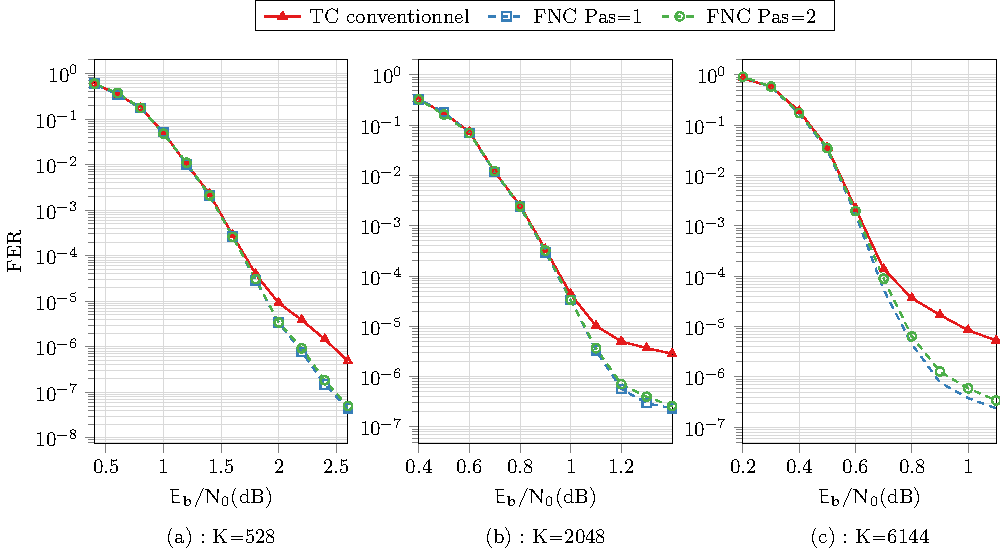
\includegraphics[width=1.1\textwidth]{main/ch4_fig/final/tikz_last/fnc10_minO_s2.pdf}
	\caption{Comparaison des performances de l'algorithme FNC appliqué toutes les deux itérations (Pas=2) ou toutes
	les itérations (Pas=1) à partir de l'itération $I_{\text{m}_\text{o}}$ pour $q=10$ et K=528,
	K=2048 ou K=6144.
	Turbo décodeur basé sur l'algorithme EML-MAP itérant au plus 8 fois.
	\label{fig:fnc_step}}
	\vspace*{-1em}
\end{figure}

En conclusion, il apparaît qu'une valeur trop faible de $I_\text{min}$ dégrade les performances de l'algorithme. 
La valeur de l'itération $I_{\text{m}_\text{o}}$ dépend des
capacités de détection du code détecteur d'erreur. L'application de l'algorithme FNC après chaque itération de turbo 
décodage permet d'obtenir les meilleures performances de décodage. Chaque suppression dans l'application du principe FNC 
dégrade les performances de décodage. Néanmoins, ne pas appliquer à chaque itération l'algorithme mais seulement une 
itération sur deux permet d'augmenter significativement le budget temps pour l'exécution de l'algorithme tout en ayant 
un impact peu significatif au niveau des performances de décodage. 
%Ceci permettra donc de réduire la complexité matérielle de 
%l'implémentation de l'algorithme FNC et sera détaillé dans une section prochaine de ce chapitre.

\subsection{Variation du nombre de mots candidats considérés}
Il a été introduit dans le chapitre précédent que les performances de l'algorithme FNC sont fortement conditionnées
par la taille du vecteur de recherche des positions probablement erronées $q$. En effet, incrémenter $q$ de $1$ revient 
à considérer deux fois plus de mots candidats. Ceci augmente de fait la probabilité d'identifier le bon mot de code. 
Cependant, la complexité calculatoire double également pour chaque incrément de $q$. En effet, il est alors nécessaire
de générer deux fois plus de mots candidats. Ceci implique un doublement du nombre de vérifications de CRC. Enfin,
l'étape de tri est elle aussi impactée. Pour ces raisons, il est nécessaire de minimiser la valeur de $q$

\begin{figure}[!t]
	\hspace*{-.075\textwidth}
	\includegraphics[width=1.1\textwidth]{main/ch4_fig/final/tikz_last/fnc_qX.pdf}
	\caption{Performances de l'algorithme FNC appliqué toutes les itérations à partir de l'itération $I_{\text{m}_\text{o}}$ pour différentes
	valeurs de $q$ et K=428, K=2048 et K=6144.
	Turbo décodeur basé sur l'algorithme EML-MAP itérant au plus 8 fois.
	\label{fig:fnc_q}}
\end{figure}

La Figure \ref{fig:fnc_q} présente l'impact de l'évolution de la valeur de $q$ pour les turbo codes du standard LTE 
d'une taille de trame allant de K=528 à K=6144. Dans tous les cas, l'algorithme FNC est utilisé toutes les itérations à 
partir de l'itération $I_\text{min} = I_{\text{m}_\text{o}}$ de telle sorte que les performances de décodages 
soient les meilleures pour $q=10$. Dans l'ensemble, comme attendu, il apparaît que la réduction de $q$ impacte 
négativement les performances de décodage. Cependant, cet impact dépend du turbo code considéré. Par exemple, pour 
$K=528$, le passage de $q=10$ à $q=8$ a un impact plus défavorable que le passage de $q=8$ à $q=6$. 
En effet, la réduction de $q=10$ à $q=8$ dégrade d'un facteur 2 les performances de décodage en terme de FER. Cette dégradation n'est que 
d'un facteur $1,2$ pour le passage de $q=8$ à $q=6$.
Ceci s'explique par
la distribution des erreurs binaires de ce turbo code. 
% En effet, une part non négligeable des trames erronées contiennent
% 9 erreurs (cf. Figure \ref{fig:be}). 
D'après la Figure \ref{fig:be} du chapitre précédent (représentant la distribution du nombre d'erreur dans la zone du 
plancher d'erreurs), $15\%$ des trames erronées possèdent exactement 9 erreurs binaires. 
Elles ne peuvent donc être corrigées que pour $q\geq 9$. 
En revanche, pour $K=2048$, la majorité des trames erronées contiennent strictement moins de 6 erreurs binaires.
%Ceci explique la similitude des performances de décodage pour une valeur de $q$ comprise entre 10 et 6 
Il apparaît alors que le passage de $q=10$ à $q=6$ ne réduit que d'un facteur 2 les performances de décodage alors que 
16 fois moins de mots candidats sont considérés.
% Cependant, le 
% passage de $q=6$ à $q=4$ impacte plus négativement les performances de décodage de l'algorithme FNC.
Enfin, pour K=6144, la situation est relativement similaire.

Finalement, il apparaît que la valeur de $q$ proposant le meilleur ratio entre amélioration des performances de décodage 
dépend fortement du turbo code considéré. Plus la valeur de $q$ est grande, meilleures sont les performances. Cependant,
avoir des valeurs de $q>9$ n'apportent que des gains marginaux pour les trois codes considérés. Ceci serait à nuancer dans le contexte 
d'un autre standard considérant un code CRC possédant de meilleures propriétés en terme de distance.

Le dernier vecteur de modifications de l'algorithme FNC en vue de son implémentation matérielle concerne la représentation de 
l'information en virgule fixe. Ceci est l'objet de la prochaine section.

\subsection{L'algorithme FNC et la quantification de l'information}
Jusqu'alors, les informations manipulées par le turbo décodeur utilisent une représentation en virgule flottante. Dans cette section, 
il est vérifié que l'algorithme FNC fourni des performances semblables lorsque la dynamique et la précision des données manipulées par
le turbo décodeur est contrainte. Pour ce faire, une étude de la dynamique des métriques $\Delta$ est mené car elle impacte
la complexité des opérations utilisées lors du tri.

Dans un premier temps, il est nécessaire de vérifier que l'algorithme FNC supporte le passage en virgule fixe des informations
manipulées par le turbo décodeur. Pour ce 
faire, les performances de décodages sont comparées suivant le format des données internes aux turbo décodeurs. 
Afin de mener cette étude, l'outil de simulation de chaîne de communications numériques AFF3CT a été utilisé.\footnote{AFF3CT : A Fast Forward Error Correction Tool est sous licence MIT et est téléchargeable depuis \url{http://aff3ct.github.io}. L'ensemble des propositions décrites dans ce manuscrit y sont intégrées.} Cet outil 
open-source supporte de nombreuses configurations permettant notamment de répondre aux contextes du standard LTE. Le 
turbo décodeur logiciel décrit permet d'obtenir parmi les meilleurs débits de la littérature \citemine{symp2}. 
Cet outil de simulation de chaîne de communications numériques permet une liberté totale sur la quantification des 
donnés du canal. Dans la suite, la notation pour la quantification de l'information est $Q_{n.d}$, avec $n$ le nombre de bits au total
et $d$ le nombre de bits utilisés pour coder la partie fractionnaire. Les formats de données pouvant être considérés pour 
le turbo décodeur sont quant à eux limités à trois. Il s'agit soit d'une représentation flottante de l'information, 
soit d'une quantification des données internes sur 16 bits, soit enfin, d'une quantification sur 8 bits.
Les performances de décodage sur 16 bits sont très proches de celles obtenues avec une 
représentation flottante de l'information. En revanche, en limitant la quantification des données 
à 8 bits, la quantification des données du canal à un impact fondamental sur les performances de décodage.
En effet, si les données du canal utilisent 5 bits au total dont 2 pour la partie fractionnaire 
($Q_{5.2}$), alors les performances de décodage dans la zone convergence sont proches de la représentation flottante. 
Cependant, le plancher d'erreurs apparaît plus tôt. Il est situé une ordre de grandeur au dessus. Dans le cas où les 
données du canal utilisent la représentation $Q_{5.1}$, la dégradation des performance de décodage se situe dans la zone 
de convergence et représente environ 0.2 dB. En revanche, pour 
les plus hautes valeurs de SNR considérées, les performances de décodage rejoignent celles obtenues dans le cas d'une 
quantification sur 16 bits. Ainsi avec cette dernière configuration, les performances dans la zone du plancher 
d'erreurs sont proches. Cette différence de performances s'explique par la nature itérative du processus de turbo 
décodage. Il apparaît que la précision a un impact sur la convergence alors que la dynamique a un impact sur le plancher d'erreurs.
%En effet, cette particularité implique un accroissement général des métriques internes lors du décodage pouvant
%amener des problématiques de dynamique complexes. 

\begin{figure}[!t]
	%\vspace*{-.5cm}
	\centering
	\hspace*{-.1\textwidth}
	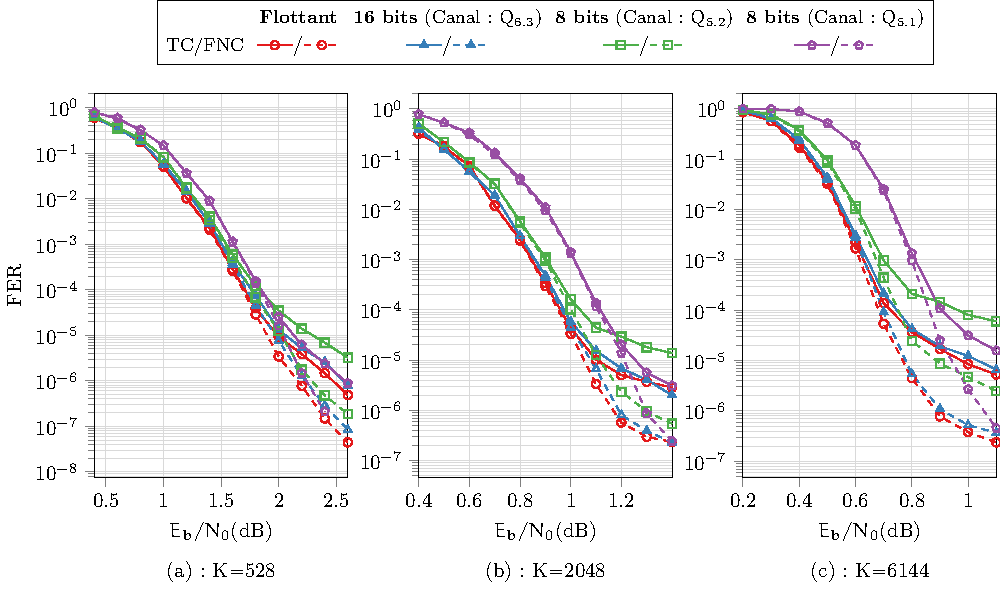
\includegraphics[width=1.1\textwidth]{main/ch4_fig/final/tikz_last/fnc10_format_refs_3.pdf}
	\caption{Comparaison des performances de l'algorithme FNC $q=10$ 
	suivant la représentation de l'information choisie, pour différents turbo codes du standard LTE.
	Turbo décodeur basé sur l'algorithme EML-MAP itérant au plus 8 fois.
	\label{fig:fnc_format_refs}}
	\vspace*{-1ex}
\end{figure}

Les performances de décodage en activant ou non le principe FNC sont récapitulées en Figure \ref{fig:fnc_format_refs} pour
ces différents contextes. 
En ce qui concerne les performances de décodage obtenues avec l'algorithme FNC, il est remarquable que quelque soit le 
choix de la représentation de l'information, les gains dans la zone de convergence atteignent ou dépassent un ordre de 
grandeur. Ainsi, il apparaît que l'algorithme FNC est robuste vis-à-vis d'une représentation en virgule fixe. Plus encore, les
gains qu'il apporte ne sont pas conditionnés par les choix de quantification réalisés au sein du turbo décodeur.

% Il apparaît alors que le passage en représentation à virgule fixe 
% induit une dégradation des performances de décodage du turbo décodeur conventionnel en regard des celles obtenues avec 
% une représentation flottante. Cette dégradation est très légère dans le cas d'une limitation à 16 bits. Elle est un peu 
% plus marquée dans le cas où les données sont sur 8 bits. \textcolor{blue}{Cette même dégradation apparaît lors de 
% l'emploi du principe FNC avec une représentation des données en virgule fixe. Ainsi, les gains en performance de 
% décodage sont conservés malgré le changement de représentation de l'information.}


\begin{figure}[!t]
	\hspace*{-.075\textwidth}
	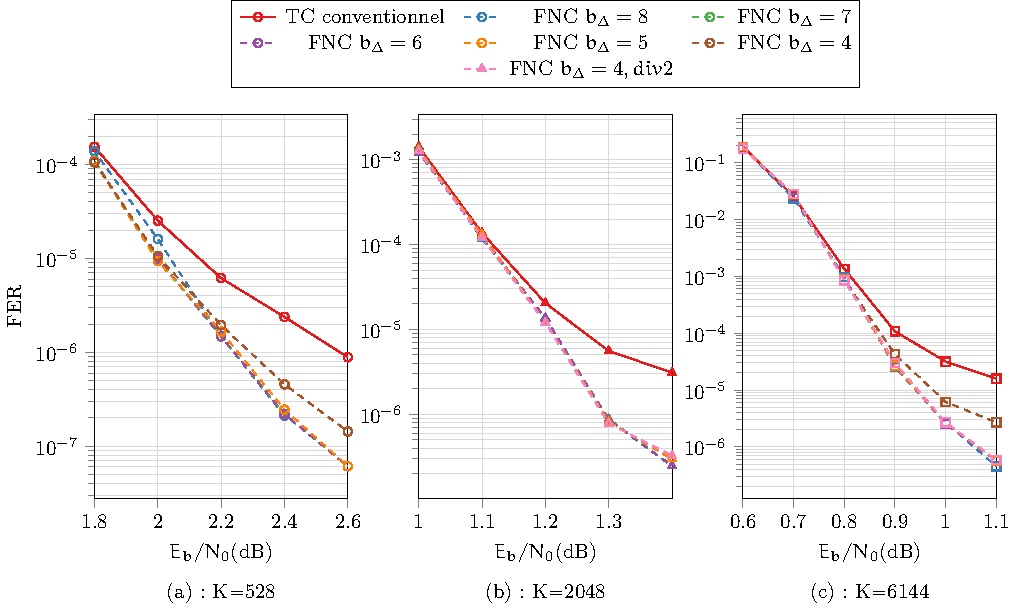
\includegraphics[width=1.1\textwidth]{main/ch4_fig/final/tikz_last/fnc10_format_8b.pdf}
	\caption{Performances de l'algorithme FNC pour différents turbo codes du standard LTE, selon la quantification $b_{\Delta}$ 
	de la métrique $\Delta$.
	Turbo décodeur 8 bits, informations du canal sur 5 bits ($Q_{5.1}$), basé sur l'algorithme EML-MAP itérant au plus 8 fois.
	\label{fig:fnc_format_8b}}
\end{figure}

Au sein de l'algorithme FNC, un tri des bits décodés est réalisé afin d'identifier les positions les moins fiables. La
complexité calculatoire de ce tri est fonction de $q$. Cependant, la dynamique de $\Delta$ influe elle aussi sur la
complexité calculatoire. En conséquence, réduire la dynamique de $\Delta$ doit permettre d'observer certains avantages.

Comme la métrique $\Delta$ de l'algorithme FNC est basée sur la valeur absolue d'une somme, sa dynamique et sa précision restent identique 
à celles des opérandes. Or, comme ce sont les valeurs minimales de la métrique $\Delta$ qui sont exploitées, il est possible de 
saturer la dynamique des données sans impacter les performances d'identification. Ceci est démontré en Figure 
\ref{fig:fnc_format_8b}. Dans tous les cas, le turbo décodeur manipule des données sur 8 bits et les données du canal 
sont sur 5 bits ($Q_{5.1}$). L'algorithme FNC est appliqué à chaque itération à partir de l'itération $I_{\text{m}_\text{o}}$. Le 
nombre de bits utilisés pour la métrique $\Delta$, noté $b_{\Delta}$ varie de 8 à 4 bits. Il 
apparaît alors que lorsque $b_{\Delta}$ vaut 8, 7, 6 ou 5 bits les performances de décodage sont équivalentes pour les trois tailles de trame considérées. À partir de $b_{\Delta} = 4$ bits une dégradation des 
performances de décodage apparaît. Cette dernière peut être réduite en effectuant une division par deux de la métrique
avant d'effectuer la saturation. 
%\textcolor{blue}{\bsc{A Vérifier : }Plus encore, effectuer une division par 4 de la métrique avant
%sa saturation sur uniquement 3 bits permet d'obtenir encore des performances équivalentes. En revanche, sur deux bits 
%les gains apportées par l'algorithme FNC s'amenuisent}

En revanche dans le cas où 16 bits sont utilisées pour la dynamique des données internes au turbo décodeur, 6 bits sont 
nécessaires à la représentation de la métrique $\Delta$ afin d'obtenir des performances de décodage identiques à celles obtenues sans saturation.



% En conclusion, pour un turbo décodeur utilisant 8 bits pour ses métriques internes, fixer la valeur de 
% $b_{\Delta}$ à 4 permet de limiter la dynamique des données en entrée de l'algorithme FNC tout en fournissant 
% des performances de décodage équivalentes à celles obtenues sans saturation.

\subsection{Conclusion}
Dans cette section, une étude de l'impact des différents paramètres de l'algorithme FNC a été menée. En effet, ces derniers ont
pour la plupart un impact notable sur les performances de décodage et la complexité calculatoire de l'algorithme FNC. 

La valeur de la profondeur de recherche $q$ doit être adaptée par le concepteur d'un turbo décodeur utilisant l'algorithme 
FNC en fonction des performances de décodage visées conjointement à l'ajout de complexité calculatoire toléré. Il en est de même 
quant au choix des itérations de turbo décodage après lesquelles appliquer l'algorithme. Le compromis peut s'exprimer comme
suit : \og Quel est le surcoût calculatoire que je suis prêt à accepter pour abaisser le plancher d'erreurs. \fg

Toutefois, il apparaît qu'il existe une valeur optimale quant à l’itération minimale. Cette valeur dépend des capacités 
de détection du code détecteur d'erreurs et donc de la taille de la trame considérée. De même, il existe une valeur de 
$\Delta_b$ permettant d'obtenir une réduction de la complexité de la fonction de tri tout en garantissant les performances de 
décodage. Cette valeur dépend essentiellement de la dynamique des informations \textit{a posteriori}.

La section suivante présente une architecture matérielle pour l'algorithme FNC dans le contexte d'un turbo décodeur 
séquentiel basé sur l'ordonnancement Backward-Forward-Sliding-Window. L'impact de 
la variation du paramètre clef $q$ sur la complexité matérielle est étudié. 


%%%%%%%%%%%%%%%%%%%%%%%%%%%%%%%%%%%%%%%%%%%%%%%%%%%%%%%%%%%%%%%%%%%%%%%%%%%%%%%%%%%%%%%%%%%%%%%%%%%%%%%%%%%%%%%%%%%%%%%%
\section{Implémentation matérielle de l'algorithme FNC}
Cette section présente une architecture matérielle pour l'algorithme FNC. Cette architecture se doit de 
s'adapter aux architectures matérielles de turbo décodeurs existants, afin d’abaisser le plancher d'erreurs des différents turbo codes présents dans 
les standards de communications numériques actuels. Cependant, il a été vu dans la première section de ce chapitre qu'une 
grande diversité dans les choix architecturaux pour les turbo décodeurs est possible. Cette section se focalise sur 
 une architecture adaptée à l'ordonnancement BF-SW, correspondant à un cas de référence. Dans un second temps, des projections
 sont faites quant à l'adaptation de cette architecture matérielle à des turbo décodeurs plus 
complexes et plus rapides. 
Afin de mener cette étude architecturale, 
le choix est fait de considérer une application de l'algorithme FNC toutes les itérations. Il a été vu dans la section 
précédente que ceci permet d'obtenir les meilleures performances de décodage avec l'algorithme FNC.

\subsection{Principe et ordonnancement de l'architecture matérielle développée}
L'algorithme FNC est un algorithme de post-traitement en regard des calculs des décodeurs SISO. En effet, l'information 
\textit{a posteriori} doit être obtenue pour pouvoir calculer la métrique $\Delta$, qui est le point d'entrée de l'algorithme FNC. Cependant, durant les 
opérations de l'algorithme FNC, le processus de turbo décodage se poursuit en parallèle. 
% Afin de 
% limiter l'impact sur la latence du décodeur, si une application de l'algorithme FNC est considérée après chaque 
% itération de turbo décodage, dans le cas d'un turbo décodeur exploitant un ordonnancement BF-SW, 
% % avec une taille de 
% % fenêtre la plus petite possible ($W\rightarrow 0$), 
% le processus FNC doit être effectué en $2\times (K+K/W)$ cycles d’exécution. 
Dans le cas d'un turbo décodeur exploitant un ordonnancement BF-SW, la durée d'une itération équivaut à  $2\times (K+K/W)$ cycles d’exécution
(pour rappel, $W$ est le nombre de fenêtres). 
Ainsi, si une application de l'algorithme FNC est considérée après chaque itération de turbo décodage, la
durée de traitement FNC ne doit pas excéder  $2\times (K+K/W)$ cycles d’exécution.
Afin d'être compatible avec n'importe quelle taille de 
fenêtre de traitement, la taille de fenêtre la plus petite possible est considéré. Cela revient à considérer un nombre 
infini de fenêtres glissantes  ($W\rightarrow \infty$). Ainsi, un temps d'exécution de $2\times K$ cycles est visé.
Ceci est 
représenté par la Figure \ref{fig:fnc_tc}. Dans ce scénario, l'architecture matérielle de l'algorithme FNC est sur-contrainte 
car un turbo décodeur utilisant l'ordonnancement BF-SW nécessite légèrement plus de $2\times K$ cycles pour 
effectuer une itération de turbo décodage. Cependant, cette architecture matérielle de référence pourra 
être améliorée ultérieurement afin de tirer parti de ces quelques cycles d'exécution supplémentaires. 

\begin{figure}[!t]
	\centering
	\includegraphics{main/ch4_fig/ipe/fnc_tc.pdf}
	\caption{Ordonnancement du système représentant les interactions entre le processus FNC et le turbo décodeur conventionnel. 
	\label{fig:fnc_tc}}
\end{figure}

\begin{figure}[!t]
	\centering
	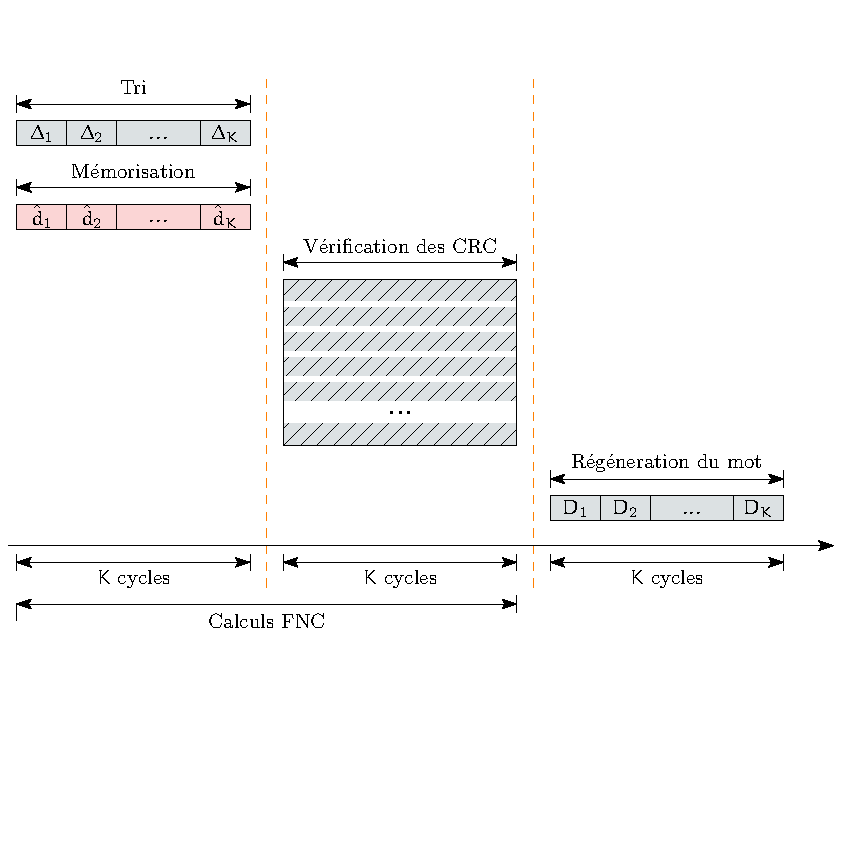
\includegraphics{main/ch4_fig/ipe/fnc_schedul.pdf}
	\caption{Ordonnancement des opérations successives au sein de l'architecture FNC. \label{fig:fnc_schedul}}
\end{figure}

La Figure \ref{fig:fnc_schedul} présente l'ordonnancement des opérations 
réalisées par l'architecture matérielle associée à l'algorithme FNC.
En accord avec la Figure \ref{fig:fnc_tc}, l'algorithme FNC est appliqué à partir de l'itération $i$. Durant les K 
premiers cycles d'exécution, le 
décodeur SISO fournit au bloc FNC la métrique $\Delta$ conjointement avec le mot décidé $\hat{d}$. 
% Le \textit{trieur 
% $\Delta$} trie alors les métriques $\Delta$ afin d'extraire les $q$ positions les moins fiables. 
Afin de conserver les $q$ positions des décisions $\hat{d}$ les moins fiables, le tri des métriques $\Delta$ est réalisé 
à la volée lors de la réception de ces informations via un module nommé \textit{trieur}. En effet, dans le cas de 
l’ordonnancement BF-SW, les K métriques $\Delta$ sont fournies séquentiellement durant K cycles d'exécution. Parallèlement, 
le mot décidé par le turbo décodeur $\hat{d}$ est mémorisé dans la \textit{mémoire de bits décidés}. Ces données permettent de générer lors de 
l'étape suivante les $2^q$ mots candidats. La génération est réalisé lors des K cycles suivants par le 
\textit{générateur de mots}. Ce dernier se base pour cela sur les bits mémorisés $\hat{d}$ ainsi que sur les $q$ positions
des minimums fournis par le module trieur.
Les 
$2^q$ mots candidats sont produits à la volée et transmis aux \textit{unités de vérification de CRC}. Finalement, au 
bout de K cycles, si un mot 
vérifiant le CRC est trouvé, ce mot est régénéré et constitue la sortie du bloc FNC. Cette régénération permet d'éviter 
le stockage des $2^q$ mots candidats. Ainsi, si un mot de code validant le
code CRC est trouvé, le processus FNC requiert au total $3\times K$ cycles d'exécution, après lesquels le processus de 
turbo décodage est stoppé. Le schéma bloc présentant l'interconnexion entre les 
différentes unités de cette solution architecturale est fourni en Figure \ref{fig:fnc_arch}. 

\begin{figure}[!t]
	\centering
	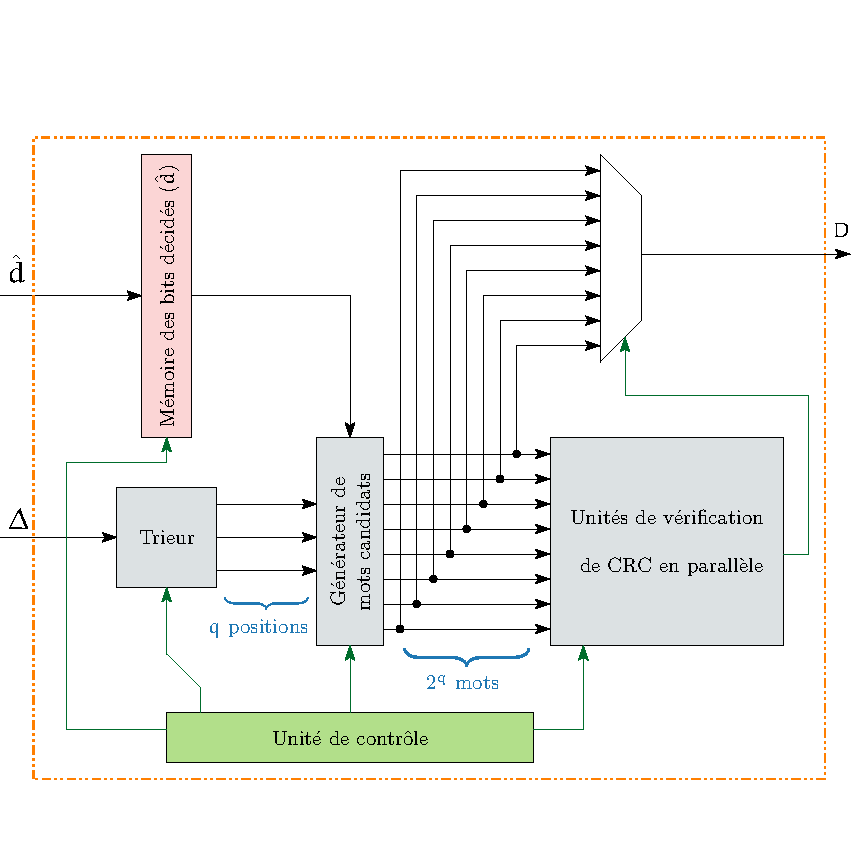
\includegraphics{main/ch4_fig/ipe/fnc_arch.pdf}
	\caption{Interconnexion des différentes unités de l'architecture FNC. \label{fig:fnc_arch}}
\end{figure}

\subsection{Détail des unités composant l'architecture matérielle FNC}
Dans cette sous-section, les différentes unités composant l'architecture matérielle pour l'algorithme FNC sont détaillés.

\paragraph*{Mémoire des bits décidés} Le principe de l'algorithme FNC est de générer $2^q1$ mots candidats à partir 
du mot décidé à l'itération courante par le turbo décodeur $\hat{d}$. Cependant, cette génération n'est possible 
qu'après avoir effectué l'identification des $q$ positions les moins fiables dans le mot décidé $\hat{d}$. C'est pourquoi ce dernier doit 
être mémorisé. Cette unité peut être implémentée au sein d'une mémoire simple port de taille $K$. Puisque les données en 
mémoire sont écrites et lues de manière ordonnée, il est aussi possible d'implémenter cette unité au sein d'un registre à décalage 
de profondeur $K$.

\paragraph*{Trieur de métrique $\Delta$} De même que les décisions $\hat{d}_i$ du turbo décodeur, une nouvelle métrique $\Delta_i$ 
est fournie à chaque cycle d'exécution. Afin de trier ces métriques au
fil de l'eau, un tri par insertion est utilisé. La nouvelle valeur de la métrique $\Delta$ est alors successivement 
comparée avec les valeurs correspondant aux $q$ positions les moins fiables. Suivant le résultat de ces comparaisons, 
les valeurs de $\Delta$ et leur positions associées sont potentiellement mises à jour. La complexité matérielle de cette unité dépend donc 
à la fois de $q$ et de la quantification de $\Delta$ (pour rappel, noté $\Delta_b$). Il a été vu que 4 bits 
pour $\Delta_b$ permet d'assurer une imperceptible dégradation des performances de décodage. Finalement, pour 
l'implémentation de ce bloc, un effort de 
$q\times(\Delta_b + \lceil log_2{K} \rceil)$ bits de mémorisation est nécessaire. Les éléments de calcul consistent 
essentiellement en $q$ comparateurs d'une taille de $\Delta_b$ bits interconnectés à un réseau de multiplexeurs.

\paragraph*{Générateur de mots candidats} Cette unité génère séquentiellement (bit à bit) tous les mots candidats en 
même temps, en combinant le mot décodé et les positions des bits les moins fiables. Pour ce faire, lorsque la position 
du bit courant coïncide avec une position minimisant la métrique $\Delta$, alors la valeur de ce bit est inversée avant d'être
transmise à l'unité de vérification des codes CRC (c'est-à-dire qu'un 1 devient un 0 et inversement). Ceci peut être 
implémenté en utilisant $2^q$ portes \bsc{ou-exclusif} dont 
une des entrées est commandée par un réseau de portes \bsc{ou} comparant la position courante et les positions les moins 
fiables. Ainsi, la complexité matérielle est conditionnée par le choix de la valeur de $q$ et $\log_2(K)$.

\paragraph*{Unités de vérification de CRC en parallèle} Puisque le choix a été fait d'assurer les vérifications 
des $2^q$ mots candidats en K cycles d'exécution, $2^q$ décodeurs de CRC séquentiels sont implémentés en parallèle.
Conformément au polynôme générateur du code CRC du standard LTE ($g_{CRC24A}$), chaque détecteur CRC nécessite 24 
\bsc{D Flip-Flop} et 13 portes \bsc{ou-exclusif}. En effet, un code CRC est basé sur un registre à décalage à rétroaction 
linéaire (LFSR) dont la boucle de retour consiste en des opérations ou-exclusif entre le bit d'entrée et les valeurs de
certaines  
\bsc{D Flip-Flop}. La complexité calculatoire de cette unité dépend de $q$, suivant une loi 
exponentielle.

\paragraph*{Unité de contrôle} La dernière unité consiste en  une machine à 3 états permettant de 
déterminer la phase courante du processus FNC. Pour rappel, celles-ci sont : 
\begin{itemize}
	\item la réception des données et le tri des métriques $\Delta$,
	\item la vérification des différents mots candidats par les décodeurs de CRC et
	\item la régénération du mot de code valide.
\end{itemize}
Aussi, 
cette unité a pour rôle majeur de mettre à jour un compteur permettant à chaque unité d'avoir connaissance de la position 
courante dans 
le mot du bit en train d'être exploité.

La section suivante présente des résultats d'implémentations de cette architecture matérielle sur une cible FPGA 
(Field-Programmable Gate Array, ou réseau de portes programmables)

\subsection{Résultats d'implémentation sur circuit FPGA}
Des résultats d'implémentation après placement et routage sur circuit FPGA sont détaillés dans cette section. L'architecture 
matérielle  présentée en Figure \ref{fig:fnc_arch} a été décrite en VHDL. 
Cette description est générique pour les paramètres $q$, $K$ et $\Delta$. Cela signifie que l'architecture FNC peut être générée pour n'importe 
quelle taille de trame de turbo code binaire et n'importe quel nombre de positions les moins fiables identifiées. Dans
tous les cas, 
l'architecture générée est conforme au bit près avec le modèle logiciel ayant permis d'obtenir les courbes de 
performances présentées au cours de ce chapitre.

Pour la plus grande valeur de K du standard LTE (K=6144) un seul bloc RAM est nécessaire pour stocker le mot décidé $\hat{d}$ 
au sein du circuit FPGA. Ainsi, 
l'architecture matérielle proposée ne nécessite qu'un seul bloc RAM, ce quelle que soit la taille de trame considérée. Dans la 
suite, seul le cas K=6144 est considéré car il correspond au cas le plus complexe.

La valeur de $\Delta_b$ est fixée à 4 bits dans un premier temps. Cette valeur permet de ne pas avoir de dégradation de 
performances de décodage pour un turbo décodeur manipulant en interne des données quantifiées sur 8 bits. Ce format 
de quantification permet de minimiser le chemin critique de la fonction de trie de la métrique $\Delta$. Ceci sera conforté par des données concernant la fréquence maximale d'exécution.

Les performances de décodage de l'algorithme FNC dépendent de la valeur du paramètre $q$. Il en est de même pour la
complexité matérielle de l'architecture décrite. Le tableau \ref{tab:fnc_impl_res_4} présente les résultats 
d'implémentation pour une cible matérielle \bsc{Xilinx Virtex-6} \bsc{xc6vlx75t-1} pour plusieurs valeurs de $q$. Ces
résultats ont été obtenus grâce à l'outil \bsc{ISE 14.7}. Les paramètres de l'outil pour les options de synthèse logique
et de placement-routage sont celles par défaut afin de faciliter la reproductibilité des résultats. La Figure \ref{fig:fnc_impl_res} présente une partie de ces résultats de façon graphique.

\begin{table}[!tb]
	\centering
	\caption{Résultats après Placement-Routage pour l'architecture associée à l'algorithme FNC (K=6144, 
	$\Delta_b = 4$ et différentes valeurs de $q$ pour le circuit FPGA \bsc{Xilinx Virtex-6} \bsc{xc6vlx75t-1}). }
	\label{tab:fnc_impl_res_4}
	\begin{tabular}{lrrrrr} 
		\toprule
		$q$ & LUT   & FF    & Slices & BRAM & f (MHz) \\ 	\cmidrule(r){1-1}\cmidrule(l){2-6}
		4   &  533  &  539  & 610    & 1	& 293     \\
		5   &  849  &  940  & 1038   & 1	& 230     \\
		6   & 1438  & 1725  & 1844   & 1    & 216     \\
		7   & 2302  & 3278  & 3127   & 1	& 207     \\
		8   & 4283  & 6267  & 5731   & 1    & 172     \\
		9   & 7970	& 12528 & 10850  & 1    & 132     \\
		10  & 15193 & 24833 & 23720  & 1    & 103     \\
		\bottomrule \vspace*{1em}
	\end{tabular}
\end{table}

\begin{figure}[!hbt]
	\centering
	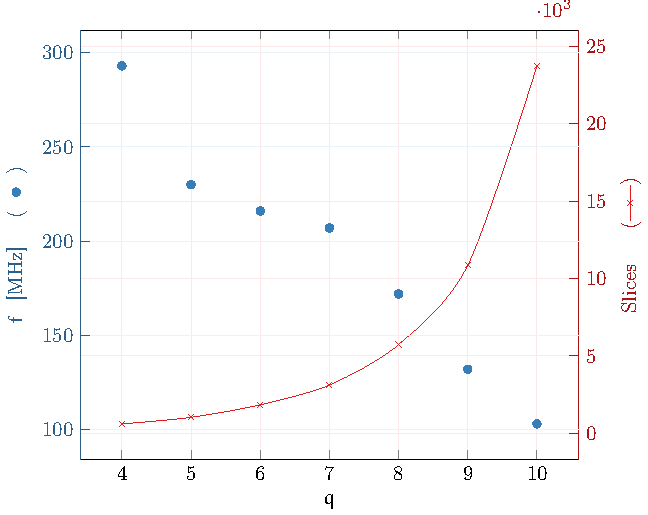
\includegraphics{main/ch4_fig/implem/xc6_4.pdf}
	\caption{Évolution de la fréquence maximale de fonctionnement et du nombre de Slices utilisées en fonction de $q$.
	Courbes réalisés en fonction des données du tableau $4.2$. \label{fig:fnc_impl_res}}
\end{figure}

Comme attendu, il apparaît que le nombre de ressources matérielles nécessaires croît exponentiellement avec $q$. 
A chaque incrément
de $q$, les ressources sont quasiment multipliées par 2. En ce qui concerne la fréquence maximale atteignable par cette 
architecture, elle décroit lorsque le nombre de mots candidats augmente. Ainsi, elle varie entre $103$ MHz pour $q=10$ 
et $293$ MHz pour $q=4$. Cette réduction de la fréquence s'explique par l'augmentation de la complexité du tri par insertion
et donc du chemin critique attenant. En effet, cette opération de tri doit être réalisé en 1 cycle d'horloge. Aussi, en 
sortie du CRC, une \bsc{réduction-en-ou} entre les sorties de toutes les unité de CRC a lieu. De part l'augmentation de
la profondeur de cette réduction avec l'augmentation de $q$, le chemin critique se voit augmenté puisque cette opération 
est elle aussi exécutée en un cycle d'horloge.

Nous allons considérer le cas $\Delta_b = 6$ pour pouvoir observer les meilleures performances de décodage avec un turbo décodeur 
utilisant une dynamique interne des données allant jusqu'à 16 bits. Les résultats de synthèse logique sont récapitulés dans le
tableau \ref{tab:fnc_impl_res_6}. Dans ce cas, il apparaît que le nombre de ressources requises augmente légèrement. La 
fréquence maximale de fonctionnement baisse de 3 à 26 MHz en fonction de la valeur de $q$. Une fois de plus, cela 
s'explique par l'augmentation de la complexité dans le tri. Comparer des données sur 6 bits implique d'augmenter la 
largeur des comparateurs et multiplexeurs. En revanche, dans le cas 
$q=10$, la fréquence augmente de 8 MHz. L'explication de cette particularité réside sans doute dans 
les heuristiques internes à l'outil Xilinx ISE. 

\begin{table}[!b]
	\centering
	\caption{Résultats après Placement-Routage pour l'architecture associée à l'algorithme FNC (K=6144, 
	$\Delta_b = 6$ et différentes valeurs de $q$ pour le circuit FPGA \bsc{Xilinx Virtex-6} \bsc{xc6vlx75t-1}). }
	\label{tab:fnc_impl_res_6}
	\begin{tabular}{lrrrrr} 
		\toprule
		$q$ & LUT   & FF    & Slices & BRAM & f (MHz) \\ 	\cmidrule(r){1-1}\cmidrule(l){2-6}
		4   & 543   & 547   & 641    & 1    & 267     \\ 
		5   & 809   & 950   & 1008   & 1    & 227     \\ 
		6   & 1465  & 1737  & 1834   & 1    & 248     \\ 
		7   & 2325  & 3292  & 3155   & 1    & 190     \\ 
		8   & 4248  & 6383  & 5973   & 1    & 163     \\ 
		9   & 8099  & 12546 & 10930  & 1    & 125     \\ 
		10  & 15432 & 24853 & 23135  & 1    & 111     \\ 
		\bottomrule 
	\end{tabular}
\end{table}

La répartition des ressources assignées selon les différentes unités (trieur, mémorisation et vérifications de CRC) est 
aussi fonction de la valeur de $q$. En effet, 
la seule unité dont la complexité croît de manière exponentielle avec $q$ est l'unité de calcul des CRC. De fait, plus $q$ prend une 
valeur élevée, plus cette unité devient prépondérante dans l'architecture. Ceci est récapitulé dans le tableau 
\ref{tab:fnc_arch_per} dont les données ont été obtenues pour une cible technologique de type ASIC tout en gardant la hiérarchie de 
l'architecture. Ainsi, pour le cas $q=10$ la quasi totalité des ressources est utilisée pour l'unité de calcul des CRC.

\begin{table}[!ht]
	\centering
	\caption{Répartition des ressources de l'architecture matérielle selon les différentes unités suivant la 
	valeur de $q$. Technologie ST 130nm}
	\label{tab:fnc_arch_per}
	% \begin{tabular}{lrrr} 
	% 	\toprule
	% 	               & $q=4$  & $q=6$  & $q=10$  \\ 	\cmidrule(r){2-2}\cmidrule(r){3-3}\cmidrule(r){4-4}
	% 	Trieur         & $21\%$ & $9\%$  & $1\%$   \\ 
	% 	Mémorisation   & $6\%$  & $2\%$  & $0.2\%$ \\ 
	% 	Calculs de CRC & $67\%$ & $74\%$ & $93\%$  \\ 
	% 	Contrôle       & $16\%$ & $8\%$  & $5\%$   \\ 
	% 	\bottomrule 
	% \end{tabular}
	\begin{tabular}{lrrrr} 
		\toprule
		 q        & Trieur  & Mémorisation  & Calculs de CRC & Contrôle  \\ 	\cmidrule(r){1-1}\cmidrule(l){2-5}
		$4$    & $21\%$ & $6\%$  & $67\%$ & $16\%$  \\ 
		$6$    & $9\%$  & $2\%$  & $74\%$ & $8\%$ \\ 
		$10$   & $1\%$ & $0.2\%$ & $93\%$ & $5\%$ \\ 
		\bottomrule 
	\end{tabular}
\end{table}

Puisque l'algorithme FNC peut être vu comme une extension d'un turbo décodeur, les résultats d'implémentation sont 
comparés avec ceux d'un turbo décodeur de la littérature. Ce dernier est disponible auprès de Xilinx sous forme d'un IP Core. 
De la sorte, il est possible d'estimer
le surcoût matériel induit par l'algorithme FNC. Le tableau \ref{tab:fnc_ip_xilinx} reporte les ressources requises
pour l'implémentation de ce turbo décodeur \cite{xilinxUMTS} sur la même cible FPGA que celle utilisée dans notre étude. 
Il apparaît que pour un contexte $q=6$, l'architecture matérielle associée à l'algorithme FNC présente un surcoût 
matériel d'environ $50\%$. Au niveau des performances de décodage, avec $q=6$ un ordre de grandeur est approché dans la 
majorité des cas pour le standard LTE. Si toutefois l'obtention de meilleures performances de décodage est visée,
l'implémentation pour $q=9$ va jusqu'à tripler le nombre de Slices. En terme de mémorisation, l'architecture matérielle 
n'a qu'un impact minime dans tous les cas puisqu'il représente moins de 10\% de surcoût. Il est 
cependant à noter qu'en l'état, cette architecture est limitante au niveau de la fréquence maximale de fonctionnement. 
Cependant, elle est sur-contrainte vis-à-vis de l'architecture de référence \cite{xilinxUMTS}. En effet, dans le cas le plus 
favorable, cette dernière effectue une itération du processus de décodage en $2,2\times K$ cycles. Or, l'architecture FNC
a été contrainte de telle sorte à fournir le résultat d'un CRC en $2\times K$ cycles. Il est donc possible de revoir l'architecture 
afin de ne plus être limité en fréquence par le bloc FNC.

\begin{table}[!b]
	\centering
	\caption{Résultats de synthèse de l'architecture matérielle de turbo décodeur %\nocite{xilinxUMTS} 
	sur cible FPGA 
	Xilinx Virtex-6 xc6vlx75t-1}
	\label{tab:fnc_ip_xilinx}
	\begin{tabular}{lrrrrrr} 
		\toprule
		LUT & FF & Slices & BRAM & f (MHz)& T/P (Mbps) \\ 
		\midrule
		3712 & 4062 & 3765 & 13 & 285 & $\sim$ 17 ($I_{TC} = 8$)\\ 
		%\cite{xilinxLTE} & 4438 & 6456 & 3918 & 33 & 385 & $\sim$ 25 &  xc7vx485t\\ 
		\bottomrule 
	\end{tabular}
\end{table}

Une architecture matérielle pour l'algorithme FNC pouvant s'adapter à tout turbo décodeur basé sur un
ordonnancement BF-SW avec une taille de fenêtre aussi petite que possible a été présentée. Cette architecture permet d'obtenir 
les meilleures performances de décodage atteignables avec l'algorithme FNC dans le contexte du standard LTE. Ce travail 
a fait l'objet d'une publication en
conférence internationale avec acte \citemine{dasip}. Il est possible de réduire le nombre d'itérations sur lesquelles 
est appliqué l’algorithme FNC tout en garantissant des performances de décodage similaires (Figure \ref{fig:fnc_step}).
Ainsi, en appliquant l'algorithme FNC toutes les deux itérations et en modifiant la machine d'états de l'architecture, 
le calcul des différents CRC peut s'effectuer durant $1,5$ itérations. Ceci permettrait une réduction  par 
trois de la surface 
requise pour l'implémentation de l'unité de calcul des CRC, prépondérante dans le coût matériel de cette architecture. 
Dans la suite de cette section, des
projections quant à la transposition de cette architecture à d'autres ordonnancements de turbo décodage sont présentées.

\subsection{Projections sur d'autres ordonnancements de turbo décodeurs}
L'architecture matérielle détaillée dans la sous-section précédente est adaptée à un turbo décodage nécessitant 2K 
cycles par itération et produisant les informations \textit{a posteriori} durant K cycles à raison d'une donnée par 
cycle. Ceci correspond à un ordonnancement BF-SW avec une taille de fenêtre la plus petite possible. Cette section présente 
différentes adaptations selon l'ordonnancement de turbo décodage retenu. Pour rappel, le tableau \ref{tab:compa} récapitule
les différents ordonnancements de turbo décodage.

\paragraph*{Adaptation pour un ordonnancement de type Butterfly (BFLY)}
Dans ce cas, la durée d'une itération vaut toujours $2\times K$. Cependant, deux donnés \textit{a posteriori} sont 
fournies en même temps durant K/2 cycles. Il est alors nécessaire de scinder la mémoire de bits décidés (Figure 
\ref{fig:fnc_arch}) en deux bancs complémentaires.
Ceci permet de mémoriser deux données en parallèle : l'une s'effectuant dans l'ordre ascendant 
et l'autre selon l'ordre descendant des positions. Pour la même raison, l'unité de tri se doit d'être dupliqué. L'une
d'elle a pour rôle d'obtenir les $q$ positions les moins fiables sur l'intervalle $\llbracket 1; K/2 \rrbracket$. L'autre
effectue parallèlement la même opération sur l'intervalle $\rrbracket K/2; K \rrbracket$. De ces deux sous-ensembles de positions
les moins fiables de taille $q$, il est nécessaire de les combiner en un seul ensemble de taille $q$. Il faut alors 
effectuer un troisième tri de $q$ positions parmi $2q$. Cependant, comme les 2 listes de $q$ positions sont triées, ce 
tri supplémentaire peut être réalisé en seulement $\epsilon$ cycles d'horloge, avec $1\leq \epsilon \leq q$ en fonction
des ressources matérielles mises en œuvre. Dans le cas $\epsilon = q$, ce tri ne nécessite qu'un seul comparateur 
de taille $\Delta_b$ bits commandant un multiplexeur à deux entrées de $\lceil\log_2(K)\rceil$ bits ainsi que la 
mémorisation des $q$ positions (chacune de $\lceil\log_2(K)\rceil$ bits). En ce qui concerne l'unité de vérification des CRC, aucune modification n'est nécessaire pour
son utilisation dans le contexte de l'ordonnancement BFLY. En effet, après les étapes de tri, $\frac{3K}{2}$ cycles 
d'exécution sont disponibles avant que de nouveaux couples de données $\Delta$ et $\hat{d}$ ne soient produits par le
turbo décodeur. Finalement, uniquement une modification des unité de tri (impliquant aussi une légère modification de 
la machine d'états) de l'architecture de référence est nécessaire pour une adaptation à un turbo décodage basé sur un 
ordonnancement de type Butterfly. Dans ce cas, la Figure \ref{fig:fnc_bfly} récapitule les ressources nécessaires ainsi 
que l'ordonnancement des opérations pour une telle architecture matérielle associée à l'algorithme FNC.

\begin{figure}[!h]
	\centering
	\includegraphics{main/ch4_fig/ipe/fnc_bfly_2.pdf}
	\caption{Adaptation de l'ordonnancement de l'architecture FNC à un turbo décodage basé sur un ordonnancement de 
	type Butterfly. \label{fig:fnc_bfly}}
\end{figure}

% Il apparait alors que les deux tris, chacun réalisé sur la moitié de la trame, s'effectue sur $\frac{K}{2}$ cycles. Or, ceci a lieu lors de 
% la seconde moitié de la première demi-itération. Entre deux tris successifs, et donc entre deux itérations successives,
% il s'écoule $\frac{3K}{2}$ cycles. Ce budget de temps permet de réaliser le tri des $q$ positions parmi $2q$ et de 
% réaliser la vérification des CRC. À nouveau, la montée en fréquence de l'architecture pourra être obtenue en 
% rompant le chemin critique grâce au surplus de cycles disponibles. Finalement, uniquement une modification des unité de
% tri (impliquant aussi une légère modification de la machine d'états) de l'architecture de référence est nécessaire pour 
% l'adapter à un turbo décodeur de type Butterfly.

\paragraph*{Adaptation pour un ordonnancement de type Butterfly avec fenêtre glissante (BFLY-SW)}
Dans le cas de l'utilisation d'une fenêtre glissante, %de taille $K/W$ 
un tri supplémentaire de $q$ parmi $2\times q$  est nécessaire afin de réunir les $q$ positions identifiées sur 
chacune des fenêtres. La machine d'état doit à nouveau être modifiée pour ce contexte. La modification consiste en 
l'ajout d'un état pour cette fusion de listes ordonnées. De la sorte, une alternance a lieu entre l'état où les deux tris en parallèle sont exécutés et l'état permettant la réunion des deux listes ordonnées en une seule. L'alternance entre les deux états doit être opérée $W$ fois, $W$ étant le nombre de fenêtres glissantes considérées.
En ce qui concerne, la vérification des CRC, $K$ cycles d'exécution sont disponibles. Ainsi, aucune modification n'est 
nécessaire dans le cas d'un turbo décodage basé sur l'ordonnancement BFLY-SW. La durée durant laquelle sont 
produites les informations \textit{a posteriori} est, comme pour 
l'ordonnancement BFLY, de $\frac{K}{2}$ cycles d'exécution. Cependant, la production s'étale sur $K-\frac{K}{2W}$ cycles. 
Ceci a pour effet de réduire à $\frac{K}{W}$ le nombre de cycles 
supplémentaires disponibles. De fait, la montée en fréquence de l'architecture pourrait être très contrainte dans les cas
considérant des fenêtres de traitement de petite taille.

\paragraph*{Adaptation pour un ordonnancement de type Butterfly avec parallélisme de sous-bloc (BFLY-SB)}
\begin{figure}[!ht]
	\centering
	\includegraphics{main/ch4_fig/ipe/fnc_bfly_sb.pdf}
	\caption{Adaptation de l'ordonnancement de l'architecture FNC à un turbo décodage basé sur un ordonnancement de type 
	Butterfly avec un degré de parallélisme de 2 (BFLY-SB). \label{fig:fnc_bfly_sb}}
\end{figure}
Un parallélisme de degré $B$ est obtenu grâce à une multiplication par $B$ des ressources 
matérielles. Cela a alors pour effet de réduire la latence de traitement du même facteur. Le nombre 
des unités de tri et
de mémorisation doit être lui aussi multiplié par $B$ puisque $2\times B$ données \textit{a posteriori} sont fournies 
simultanément. Pour assurer les vérifications de CRC, il est alors nécessaire de paralléliser les unités de traitement 
de CRC. En effet, celles-ci doivent être capables de traiter les $B$ bits de la trame durant un cycle d'exécution. La valeur 
maximale usuelle de $B$ trouvée dans la littérature est 16. La Figure \ref{fig:crc_par} présente les résultats de synthèse 
logique
en équivalent porte (cible ASIC) pour une unité de vérification CRC du standard LTE. Cinq degrés de parallélisme (de 1 à 48)
sont étudiés.
Il apparaît alors que le coût de l'unité de calcul de CRC croît mais l'incrément du degré de parallélisme ne correspond pas à un 
doublement du coût matériel. Ceci est corroboré par une métrique qui correspond au calcul du degré de parallélisme divisé par le nombre équivalent
de portes \bsc{nand-2}, comme présenté dans la Figure \ref{fig:crc_par}. Cette métrique est une indication
de l'efficacité énergétique. 
Ce résultat ouvre l'opportunité d'une modification intéressante de l'architecture FNC de référence. En effet, par 
exemple, une unité séquentielle de CRC nécessite $203$ portes \bsc{Nand-2}. Pour le cas $q=10$, l'unité de vérification 
de CRC requiert alors $207669$ portes \bsc{Nand-2}. Une unité de calcul de CRC d'un degré de parallélisme de 48 nécessite 
$1055$ portes \bsc{Nand-2}. Une telle unité nécessite $K/48$ cycles d'exécution afin de vérifier un CRC. Afin d'effectuer
les 1023 calculs de CRC, en exactement K cycles d'exécution, il est alors nécessaire d'implémenter seulement 22 unités
de calcul de CRC d'un degré de parallélisme de 48. Ceci permet alors de n'utiliser plus que $23210$ portes \bsc{Nand-2}
pour implémenter l'unité de vérification des CRC. De  la sorte, l'empreinte de cette unité peut être réduite d'un facteur
9.
%Cette augmentation de l’efficacité ouvre l'opportunité d'une réduction des besoins en surface de l'architecture FNC de 
%référence. 
La Figure \ref{fig:fnc_bfly_sb} présente les ressources nécessaires ainsi que l'ordonnancement des 
opérations de l'architecture adaptée à un turbo décodeur de type BFLY-SB pour un parallélisme de 2 ($B=2$).

\begin{figure}[!tb]
	\centering
	\includegraphics{main/ch4_fig/implem/crc.pdf}
	\caption{Évolution du coût matériel de l'implémentation d'un calcul de CRC suivant le degré de parallélisme.
	Résultats de synthèses logique en équivalent portes \bsc{nand-2}. Technologie ST 130nm. Fréquence de 500MHz.}
	\label{fig:crc_par}
\end{figure}

\paragraph*{Adaptation pour un ordonnancement de type Butterfly à fenêtre glissante et avec parallélisme de sous-bloc 
(BFLY-SW-SB)}
Cet ordonnancement de turbo décodage, le plus complexe étudié dans ce chapitre consiste en la combinaison des
deux ordonnancements précédents. Une architecture matérielle adapté à un tel turbo décodage doit alors adresser 
toutes les modifications précédemment introduites. Ainsi, le nombre de tri à effectuer en parallèle est de $2\times B$. 
De ces $2\times B$ listes de
$q$ positions, $2\times B-1$ opérations de fusion doivent être réalisées afin de ne garder que les $q$ positions les moins 
fiables de la trame. Chaque unité de CRC doit être adaptée à un degré de parallélisme de $B$ afin d'effectuer 
l'ensemble des 
vérifications de CRC en $\frac{K}{B}$ cycles. Enfin, le nombre de cycles entre la fin des 
opérations de CRC et le début du prochain tri sur le nouveau jeu de donnée doit valoir $\frac{K}{2\times B\times W}$.

\paragraph*{Conclusion}
Dans cette sous-section les modifications à apporter à l'architecture FNC de référence afin de l'adapter à différents 
ordonnancement de turbo décodage ont été introduites. À la vue de ces différentes modifications, il apparaît possible 
d'adapter l'architecture FNC aux différents ordonnancements de turbo décodage. Ceci montre la polyvalence de l'algorithme
FNC quant à son implémentation. Cependant, ces synthèses ainsi que les résultats restent à mener. Le tableau \ref{tab:fnc_recap} récapitule les différentes projections sur l'architecture matérielle suivant le 
turbo décodage considéré.

\begin{table}[!t]
	\centering
	\caption{Récapitulatif des modifications requises par rapport à l'architecture de référence afin de l'adapter à 
	d'autres ordonnancements de turbo décodeurs.}
	\label{tab:fnc_recap}
	\resizebox{\textwidth}{!}{
	\begin{tabular}{lrrrr} 
	%\begin{tabular}{rllll} 
		\toprule
		             & Unité de Tri                & Mémorisation & Unité CRC & Machine d'états \\ 
		           \cmidrule(r){2-2}\cmidrule(r){3-3}\cmidrule(r){4-4}\cmidrule(r){5-5}
		\textbf{BFLY}         & $\times 2$ + 1 fusion       & 2 bancs      & --        & Tri et mémorisation  \\ 
		\textbf{BFLY-SW} (W)  & $\times 2$ + 2 fusions      & 2 bancs      & Idem BFLY & Idem BFLY + tri     \\ 
		\textbf{BFLY-SB} (B) & $\times 2B$ + (B-1) fusions & $B\times$ BFLY & Parallélisme $(B)$    & tri et mémorisation    \\ 
		\bottomrule 
	\end{tabular}}
\end{table}

\section{Conclusion}
Dans ce quatrième chapitre, une architecture matérielle de correction des erreurs résiduelles a été détaillé. 
Afin d'aboutir à cette proposition, différents ordonnancements de turbo décodage ont été présentées dans un premier temps.
Ces ordonnancements, séquentiels ou parallèles, peuvent adresser un large panel applicatif
répondant à différents contextes.

Dans un second temps, une étude quant à l'influence des paramètres de l'algorithme FNC a été menée. Il apparaît que 
ceux-ci interagissent à la fois sur la complexité calculatoire et sur les performances de turbo décodage.
Certains de ces paramètres possèdent des valeurs optimales alors que d'autres doivent être adaptés selon un
compromis entre performances de décodage et complexité matérielle résultante.

Finalement, la troisième section présente le cas d'étude d'une architecture matérielle pour l'algorithme FNC adapté à
un ordonnancement de turbo décodage particulier. Le principe, l'ordonnancement et la composition de cette architecture ont 
été détaillés. S'en est suivi des résultats d'implémentation pour une cible FPGA. Ces résultats ont été comparés à un 
turbo décodeur vendu sous forme d'IP Core par Xilinx. Finalement, des projections quant à la transposition de ce cas 
d'étude sur d'autres
types de turbo décodeur ont été menées. Ceci conforte le fait qu'une implémentation matérielle de l'algorithme FNC est
envisageable ce quelque soit le turbo décodeur considéré; afin de permettre une correction des erreurs résiduelles et
donc un abaissement du plancher d'erreurs des turbo codes.
